\documentclass[review,authoryear,12pt]{elsarticle}
\usepackage{fontspec}
\setmainfont{TeX Gyre Termes}
\usepackage{amsmath,amssymb,graphicx,booktabs,longtable,array,calc,etoolbox}
\usepackage[hidelinks]{hyperref}
\usepackage{xurl}
\usepackage{setspace}
\usepackage{needspace}
\providecommand{\tightlist}{\setlength{\itemsep}{0pt}\setlength{\parskip}{0pt}}
\providecommand{\pandocbounded}[1]{#1}
\AtBeginEnvironment{longtable}{\footnotesize\setstretch{1.0}}
\setlength{\LTleft}{0pt}
\setlength{\emergencystretch}{3em}
\journal{Finance Research Open}
\begin{document}
\begin{frontmatter}
\title{Who gains from a market upgrade? Stock liquidity and prices around
Vietnam's FTSE Russell reclassification}
\begin{abstract}
FTSE Russell reclassified Vietnam from frontier to secondary emerging
status in four public steps between October 2025 and September 2026.
Such upgrades promise new foreign demand, but studies of aggregate
indices or country-level flows do not show which stocks gain or when.
Using daily data on 366 Ho Chi Minh City Stock Exchange stocks, we trace
liquidity and prices at each step. Because FTSE chose the final
constituents on mid-2026 data, we estimate effects for the 24 eventual
constituents and, as an intention-to-treat design, for the 27 stocks
FTSE had screened as eligible on data from before the announcement.
Relative to never-named stocks, the Amihud illiquidity of the
pre-announcement eligible group fell by 24\%, 43\% and 56\% after the
announcement, the confirmation and the constituent list; for the
constituents the declines were 32\%, 59\% and 68\%. Constituents earned
cumulative abnormal returns of 3.9\% to 7.8\% in the announcement week
and 2.7\% to 4.5\% around the confirmation, significant under four
benchmarks and a test that allows for the common event dates; the
constituent list and the first 10\% index tranche produced no reliable
price effect. Trading value surged at the rebalancing close for included
stocks but not for stocks FTSE named and then excluded. The liquidity
and price responses came with FTSE's disclosures, before index funds had
to buy.
\end{abstract}
\begin{keyword}
market reclassification \sep index effect \sep stock liquidity \sep frontier markets \sep intention to treat \sep Vietnam
\JEL G12 \sep G14 \sep G15
\end{keyword}
\end{frontmatter}
\doublespacing
\hypertarget{introduction}{%
\section*{1. Introduction}}

The liquidity of likely index stocks improved from the announcement of
Vietnam's market upgrade onward, before index funds had to buy. Relative
to never-named stocks on the Ho Chi Minh City Stock Exchange (HOSE), the
Amihud (2002) illiquidity of the 27 stocks FTSE Russell had screened as
eligible on 2024 data fell by 43\% after the April 2026 confirmation and
by 56\% after the August 2026 constituent list. For the final
constituents, the declines were 59\% and 68\%. At the first index
tranche, prices showed no reliable change, while trading value surged at
the rebalancing close for included stocks only.

Market classification decides which benchmarks a country's stocks can
enter, and benchmark weights steer international portfolio allocations
(Raddatz et al., 2017). An upgrade to emerging status therefore promises
new foreign demand. Because liquidity is priced in emerging markets
(Bekaert et al., 2007), the cost of capital of issuers depends in part
on which stocks that demand reaches, and when.

Existing evidence says little about this for frontier markets. Additions
to the S\&P 500 raise trading activity and narrow spreads persistently
(Hegde \& McDermott, 2003). In frontier markets, index additions raise
prices persistently, and Biktimirov and Afego (2026) attribute the gains
to institutional demand. Studies of market reclassification mostly use
aggregate indices or country-level flows (e.g., Burnham et al., 2018;
Raddatz et al., 2017), which pool all stocks and so cannot separate the
stocks an upgrade targets from market-wide trends. An earlier study of
the same market by the present authors (anonymized for review) found no
structural breaks in index-level liquidity at FTSE watch-list reviews
but could not identify which stocks gained.

Vietnam's reclassification offers a cleaner test. FTSE disclosed it in
four dated steps, each resolving a different uncertainty: the
announcement (7 October 2025), the confirmation (7 April 2026), the
constituent list (21 August 2026) and the effective date (21 September
2026). Hundreds of HOSE stocks outside the index form a comparison
group. FTSE also published a preliminary list of eligible stocks
screened on data as of 31 December 2024, before the announcement, which
supports intention-to-treat (ITT) estimates that do not depend on its
later choice. That choice used liquidity data up to June 2026 (FTSE
Russell, n.d.), in the middle of our sample, so comparing final
constituents with other stocks could mistake selection for an upgrade
effect. We therefore drop from the comparison group every stock FTSE
named as eligible but did not include.

We estimate difference-in-differences and event-study regressions on
35,752 stock-weeks and on daily returns from October 2024 to September
2026. The main liquidity measure is the Amihud ratio on traded value in
Vietnamese dong (VND); we also report trading value, the Corwin and
Schultz (2012) high-low spread (CS spread), volatility and cumulative
abnormal returns (CARs). We test CARs at the portfolio level to account
for the common event dates (Brown \& Warner, 1985) and call them
reliable only if significant at 5\% under all four benchmarks.

We make one contribution: we decompose the stock-level liquidity and
price effects of a frontier-to-emerging reclassification by disclosure
stage, with a treatment group also fixed before the upgrade. In a search
bounded to Crossref records and the literature cited here, we found no
earlier stock-level estimate of this effect with a comparison group and
a pre-determined treatment list, and unlike Biktimirov and Afego (2026)
we follow liquidity stage by stage within one market. Four findings
support the decomposition. First, the illiquidity of the ITT group fell
by 0.27, 0.55 and 0.81 log points across the three windows, about two
thirds of the constituent declines; for constituents, the confirmation
brought a discrete step beyond a gradual post-announcement drift, and
the constituent list did not (Section 4.1). Second, prices rose reliably
in the announcement week and at the confirmation, and the confirmation
gain persisted under three of four benchmarks (Section 4.2). Third,
trading value surged by 0.79 log points at the rebalancing close, rising
with FTSE size segment, with no surge for named-but-excluded stocks
(Sections 4.3 and 4.4). Fourth, FTSE's eligibility lists partly followed
rising liquidity (Section 5.2), which limits causal readings of the
constituent estimates.

The remainder of the paper is organized as follows. Section 2 describes
the setting, reviews the literature and states the hypotheses. Section 3
presents the data and design, Section 4 the results and Section 5 the
robustness checks and the selection evidence. Section 6 concludes.

\hypertarget{setting-literature-and-hypotheses}{%
\section*{2. Setting, literature and
hypotheses}}

\hypertarget{ftse-russells-four-step-reclassification-of-vietnam}{%
\subsection*{2.1 FTSE Russell's four-step reclassification of
Vietnam}}

FTSE Russell added Vietnam to its watch list in September 2018 (FTSE
Russell, 2018). On 7 October 2025 it announced an upgrade to secondary
emerging status effective 21 September 2026, subject to an interim
review in March 2026 (LSEG, 2025), and on 7 April 2026 it confirmed the
upgrade and the date (LSEG, 2026). Inclusion is phased in tranches of
10\%, 20\%, 35\% and 35\% of the index weight on 21 September 2026, 22
March 2027, 21 June 2027 and 20 September 2027 (FTSE Russell, 2026), so
the effective date we study carried only the first tenth.

Between these dates the financial press reported FTSE's lists of
eligible stocks. A preliminary list of 28 names appeared in November
2025 (Viet Nam News, 2025); it was screened on data as of 31 December
2024 (The Investor, 2026a). A list of 32 names, screened on data as of
31 December 2025, followed in April 2026, dropping Petrolimex (PLX) and
adding BID, FPT, NVL, GEE and BSR (The Investor, 2026b). On 21 August
2026 FTSE published 27 constituents, effective after the close of 18
September 2026 (FTSE Russell, 2026; VIR, 2026) and screened on liquidity
data up to the last business day of June (FTSE Russell, n.d.). FTSE
applies liquidity, minimum-size and foreign-headroom screens, and in the
liquidity test it uses the investability weight of each security, which
reflects its free float and foreign-ownership limits (FTSE Russell,
2026). The same weight scales the index weight of a security, and each
tranche applies a fraction of it. A security with a 49\% investability
weight thus enters at 4.9\% after the first tranche (10\% of 49\%) and
at 49\% after the last, so index weight and passive demand rise with
free-float market capitalization. Appendix Table A.1 lists the stocks.

\hypertarget{index-inclusion-and-liquidity}{%
\subsection*{2.2 Index inclusion and
liquidity}}

Two channels link index membership to liquidity and prices. Under the
price-pressure channel, additions lead index funds to buy, which
produces temporary volume and price effects that reverse afterwards
(Harris \& Gurel, 1986). Under the demand and recognition channel, the
investor base changes lastingly. Shleifer (1986) interprets excess
returns that persist for at least ten days after inclusion as evidence
that demand curves for stocks slope down. Chen et al.~(2004) find
asymmetric effects of additions and deletions that fit a gain in
investor awareness, and Hegde and McDermott (2003) attribute the
persistent liquidity gains of S\&P 500 additions mainly to lower direct
trading costs.

Liquidity gains from inclusion also have real consequences: S\&P 500
additions with larger liquidity improvements increase capital investment
(Becker-Blease \& Paul, 2006), whereas the liquidity lost after FTSE 100
deletions has no significant effect on investment (Gregoriou \& Nguyen,
2010). Because liquidity co-moves across stocks (Chordia et al., 2000),
such studies must separate stock-specific changes from market-wide
liquidity shocks.

\hypertarget{market-reclassification-and-frontier-markets}{%
\subsection*{2.3 Market reclassification and frontier
markets}}

Reclassification moves a whole market between benchmark families.
Because mutual funds allocate across countries with reference to
benchmark weights, a change in classification changes capital flows
(Raddatz et al., 2017) and can move currency values (Hau et al., 2010).
Burnham et al.~(2018) show that, when MSCI moves a country to a
different index family, its stock prices move sharply in the direction
implied by the new benchmark before implementation and give back most of
that move in the following year. After MSCI included China A-shares in
its Emerging Markets Index, the included stocks earned abnormal returns
around the announcement, and market quality changed over the longer run
through liquidity, turnover and price synchronization (Dong et al.,
2023); beyond that study, we did not locate a stock-level study of
liquidity around the China A-share inclusion. Frontier-market evidence
is thinner. Biktimirov and Afego (2026) study changes to the FTSE
Frontier 50 Index from 2008 to 2025; they find persistent price gains
for additions and distinct return and trading-volume responses when a
country changes class, and they trace the gains to institutional demand
rather than to trading pressure or liquidity.

Liquidity carries particular weight in these markets. Local market
liquidity predicts returns in emerging markets, where segmentation from
global capital is only partial (Bekaert et al., 2007). Stereńczak et
al.~(2020) ask whether frontier-market investors demand compensation for
illiquidity. A liquidity gain for some stocks could therefore shift
their cost of capital, although we do not measure that shift. Vietnamese
evidence from before the upgrade concerns market-wide shocks such as the
COVID-19 outbreak (Nguyen et al., 2021), not classification events.

\hypertarget{hypotheses}{%
\subsection*{2.4 Hypotheses}}

The recognition channel predicts that liquidity and prices respond when
information reaches investors, at the announcement, the confirmation and
the constituent list; the price-pressure channel predicts a trading and
price spike when index funds rebalance, followed by reversal.

H1. After the reclassification announcement, stocks likely to enter the
index become less illiquid than other HOSE stocks.

H2. The liquidity gap widens at each later disclosure that resolves
uncertainty about the upgrade and its constituents.

H3. Likely constituents earn abnormal returns at the disclosures, and
the first index tranche adds no further price effect.

H4. The rebalancing session produces a trading-value surge for
constituents, and not for excluded stocks, that scales with index
weight.

\hypertarget{data-and-empirical-design}{%
\section*{3. Data and empirical design}}

\hypertarget{sample-and-groups}{%
\subsection*{3.1 Sample and groups}}

We collect daily open, high, low and close prices and share volume for
all 405 common stocks listed on HOSE on 24 September 2026, from 1
October 2024 to 23 September 2026, from the Vietcap Securities (VCI)
feed through the open-source vnstock library; the sample therefore omits
stocks delisted during the period. We keep stocks with at least 200
trading days before 7 October 2025, zero volume on fewer than 20\% of
those days, and a median price of at least VND 1,000, which leaves 366
stocks.

We sort the stocks into three groups (Appendix Table A.1). Constituents
are the 24 of the final 27 with a full pre-period (TCX, VPL and VCK
listed after October 2025). Named-but-excluded stocks are the 14 HOSE
stocks on the November 2025 or April 2026 eligible list that FTSE did
not include; a fifteenth, Tasco (HUT), trades on the Hanoi exchange. The
remaining 328 never-named stocks form the comparison group. The ITT
group consists of the 27 HOSE stocks on the preliminary list, 15 of
which became constituents. BSR traded on the Unlisted Public Company
Market (UPCoM) until 6 January 2025 and on HOSE from 17 January 2025
(VietnamPlus, 2024), so its pre-period spans two venues; Section 5.2
reports results without it.

Table 1 compares the groups before the announcement. Constituents traded
a mean of 6.82 log VND billion per week against 2.19 for never-named
stocks, with a mean Amihud ratio about three orders of magnitude lower,
and named-but-excluded stocks sit between the two; spreads and absolute
returns are similar. This size gap motivates the matched sample and the
size-specific checks.

\needspace{14\baselineskip}\textbf{Table 1. Pre-announcement characteristics by group, October 2024
to 6 October 2025}

\begin{longtable}[]{@{}>{\raggedright\arraybackslash}p{(\linewidth - 12\tabcolsep) * \real{0.2000}}>{\raggedright\arraybackslash}p{(\linewidth - 12\tabcolsep) * \real{0.1333}}>{\raggedright\arraybackslash}p{(\linewidth - 12\tabcolsep) * \real{0.1333}}>{\raggedright\arraybackslash}p{(\linewidth - 12\tabcolsep) * \real{0.1333}}>{\raggedright\arraybackslash}p{(\linewidth - 12\tabcolsep) * \real{0.1333}}>{\raggedright\arraybackslash}p{(\linewidth - 12\tabcolsep) * \real{0.1333}}>{\raggedright\arraybackslash}p{(\linewidth - 12\tabcolsep) * \real{0.1333}}@{}}
\toprule\noalign{}
\begin{minipage}[b]{\linewidth}\raggedright
Group
\end{minipage} & \begin{minipage}[b]{\linewidth}\centering
Stocks
\end{minipage} & \begin{minipage}[b]{\linewidth}\centering
Stock-weeks
\end{minipage} & \begin{minipage}[b]{\linewidth}\centering
Amihud
\end{minipage} & \begin{minipage}[b]{\linewidth}\centering
log trading value
\end{minipage} & \begin{minipage}[b]{\linewidth}\centering
CS spread (\%)
\end{minipage} & \begin{minipage}[b]{\linewidth}\centering
Absolute return (\%)
\end{minipage} \\
\midrule\noalign{}
\endhead
\bottomrule\noalign{}
\endlastfoot
Constituents & 24 & 1,248 & 0.00017 & 6.82 & 0.57 & 1.40 \\
Named, not included & 14 & 726 & 0.0033 & 5.96 & 0.61 & 1.49 \\
Never-named & 328 & 16,915 & 0.195 & 2.19 & 0.61 & 1.37 \\
\end{longtable}

\emph{Notes}: Weekly means, with Amihud from Eq. (1) and the
Corwin--Schultz (CS) spread from Eqs. (2)--(3). Source: Authors'
calculations.

\hypertarget{liquidity-and-return-measures}{%
\subsection*{3.2 Liquidity and return
measures}}

Daily traded value \(\mathrm{VAL}_{it}\) is the closing price times
share volume of stock \(i\) on day \(t\), in VND billion, and \(R_{it}\)
is its daily log return. Following Amihud (2002), who divides the
absolute daily return by dollar volume, we define daily illiquidity as

\[\mathrm{ILLIQ}_{it} = \frac{|R_{it}|}{\mathrm{VAL}_{it}}. \qquad (1)\]

Traded value makes the ratio comparable across price levels, and our
volume filter limits the loss of accuracy that Kang and Zhang (2014)
document for the Amihud ratio in emerging markets with many zero-volume
days. The CS spread uses the daily high \(H_{it}\) and low \(L_{it}\)
over two consecutive days (Corwin \& Schultz, 2012):

\[\phi_{it} = \left[\ln\frac{H_{it}}{L_{it}}\right]^2 + \left[\ln\frac{H_{i,t-1}}{L_{i,t-1}}\right]^2, \qquad \psi_{it} = \left[\ln\frac{\max(H_{it}, H_{i,t-1})}{\min(L_{it}, L_{i,t-1})}\right]^2, \qquad (2)\]

\[\eta_{it} = \frac{\sqrt{2\phi_{it}} - \sqrt{\phi_{it}}}{3 - 2\sqrt{2}} - \sqrt{\frac{\psi_{it}}{3 - 2\sqrt{2}}}, \qquad S_{it} = \max\left\{0,\ \frac{2\left(e^{\eta_{it}} - 1\right)}{1 + e^{\eta_{it}}}\right\}, \qquad (3)\]

where \(\phi_{it}\) sums the squared log high-low ranges of days \(t-1\)
and \(t\), \(\psi_{it}\) is the squared log range over the two days
combined, and \(S_{it}\) is the resulting spread estimate, set to zero
when negative. We winsorize \(\mathrm{ILLIQ}_{it}\) and \(S_{it}\) at
the 1st and 99th percentiles of each day and keep stock-weeks with at
least three trading days and a positive Amihud ratio. For stock \(i\) in
week \(w\) with \(N_{iw}\) trading days,

\[\begin{aligned} \mathrm{Amihud}_{iw} &= \ln\left(\frac{1}{N_{iw}}\sum_{t \in w}\mathrm{ILLIQ}_{it}\right), \\ \mathrm{TV}_{iw} &= \ln\left(\sum_{t \in w}\mathrm{VAL}_{it} + 10^{-6}\right), \qquad (4) \\ \mathrm{Vol}_{iw} &= \ln\left(\frac{1}{N_{iw}}\sum_{t \in w}|R_{it}|\right), \end{aligned}\]

and the weekly spread is the mean of \(S_{it}\) within the week.

For prices, the abnormal return of stock \(i\) on day \(t\) against
benchmark return \(R_{bt}\) is

\[\mathrm{AR}_{it} = R_{it} - R_{bt} \quad \text{or, in the market model,} \quad \mathrm{AR}_{it} = R_{it} - \left(\hat a_i + \hat b_i R_{bt}\right). \qquad (5)\]

The four benchmarks are the equal-weighted mean of the 328 never-named
stocks, the matched controls described below weighted by their matching
weights, the equal-weighted mean of the 110 never-named stocks in the
top tercile of pre-period trading value among never-named stocks, and a
market model whose \(\hat a_i\) and \(\hat b_i\) are estimated for each
stock against the first benchmark. Because constituents share event
dates, their abnormal returns are correlated, so we test CARs on the
equal-weighted portfolio \(p\) of the \(N_g\) stocks in group \(g\),
which addresses cross-sectional dependence (Brown \& Warner, 1985). With
trading days indexed by \(s\) relative to the disclosure date
(\(s = 0\)),

\[\begin{aligned} \mathrm{AR}_{ps} &= \frac{1}{N_g}\sum_{i \in g}\mathrm{AR}_{is}, \qquad \mathrm{CAR}_p(\tau_1, \tau_2) = \sum_{s=\tau_1}^{\tau_2}\mathrm{AR}_{ps}, \qquad (6) \\ t_{\mathrm{CAR}} &= \frac{\mathrm{CAR}_p(\tau_1, \tau_2)}{\hat\sigma_p\sqrt{D}}, \end{aligned}\]

where \(\tau_1\) and \(\tau_2\) are the first and last days of the event
window, \(\hat\sigma_p\) is the standard deviation of
\(\mathrm{AR}_{ps}\) in the estimation window and
\(D = \tau_2 - \tau_1 + 1\); the statistic assumes independent daily
abnormal returns. The estimation window runs from day −130 to day −11
and excludes days −1 to +20 around every earlier disclosure, which
leaves 120 estimation days for the announcement, 98 for the confirmation
and the constituent list, and 89 for the effective date. We pre-specify
the windows {[}−1,+1{]}, {[}−1,+5{]} and {[}0,+20{]} for every
disclosure, report all of them and call a CAR reliable when it is
significant at 5\% under all four benchmarks.

\hypertarget{estimation}{%
\subsection*{3.3 Estimation}}

The baseline liquidity specification is

\[y_{iw} = \alpha_i + \lambda_w + \sum_{k=1}^{3}\beta_k\left(\mathrm{Constituent}_i \times P_{kw}\right) + \varepsilon_{iw}, \qquad (7)\]

where \(y_{iw}\) is an outcome from Eq. (4) or the weekly spread for
stock \(i\) in week \(w\), \(\alpha_i\) and \(\lambda_w\) are stock and
week fixed effects, \(\mathrm{Constituent}_i\) equals one for the 24
constituents and zero otherwise, \(P_{1w}\), \(P_{2w}\) and \(P_{3w}\)
indicate the announcement window (7 October 2025 to 6 April 2026), the
confirmation window (7 April to 20 August 2026) and the
list-and-rebalancing window (21 August to 23 September 2026),
\(\beta_k\) is the change in the outcome of constituents relative to
never-named stocks in window \(k\), and \(\varepsilon_{iw}\) is the
error term. Weeks start on Monday and enter a window only if they start
on or after the disclosure date. FTSE did not state the hour at which it
released the constituent list; both the weekly assignment and the
{[}−1,+1{]} event window, which spans 20, 21 and 24 August, contain the
first Vietnamese session after the release. The comparison group
contains only never-named stocks. Week fixed effects absorb market-wide
liquidity shocks, which co-move across stocks (Chordia et al., 2000),
and we cluster standard errors by stock.

The ITT specification replaces \(\mathrm{Constituent}_i\) in Eq. (7)
with \(\mathrm{ITT}_i\), which equals one for the 27 stocks on the
preliminary list, and keeps all other stocks (in a variant, only
never-named, never-included stocks) as controls. A third treatment
group, the ``predicted constituents'', consists of the 27 stocks with
the highest pre-announcement trading value, 16 of which became
constituents. For timing, we estimate a monthly event study (Roth et
al., 2023):

\[y_{iw} = \alpha_i + \lambda_w + \sum_{m \neq -1}\delta_m\left(\mathrm{Constituent}_i \times M_{mw}\right) + \varepsilon_{iw}, \qquad (8)\]

where \(M_{mw}\) equals one if week \(w\) starts in month \(m\), counted
from October 2025 (\(m = 0\)), with \(m\) running from −13 (the week of
30 September 2024) to 11 and September 2025 (\(m = -1\)) as the omitted
month. To separate a discrete step at each disclosure from gradual
change, a drift variant adds
\(\kappa\left(\mathrm{Constituent}_i \times s_w\right)\) to Eq. (7),
where \(s_w\) counts weeks since the announcement and is zero before it;
a trend variant uses weeks since the start of the sample instead.

Because constituents are the largest HOSE stocks, we also use a matched
sample that pairs each constituent with three never-named stocks by
nearest-neighbour propensity score, with replacement, on pre-period
return volatility, price and traded value, weighting each control by its
matching weight (Ho et al., 2007). Matching reduces the standardized
mean difference (SMD) in pre-period traded value from 4.06 to 0.04
(Appendix Table A.2). A further check replaces week fixed effects with
size-tercile-by-week fixed effects. For inference with 24 treated
stocks, we report a wild cluster bootstrap with restricted residuals,
Rademacher weights and 999 draws (Cameron et al., 2008), and
randomization inference with 500 pseudo-treated groups of 24 stocks
drawn from the 85 never-named stocks in the top tercile of pre-period
trading value among all 366 stocks. Because all constituents were
treated at the same dates, adoption is not staggered, and the two-way
fixed effects estimator does not suffer the negative-weighting problem
that motivates Callaway and Sant'Anna (2021).

For the rebalancing session we estimate, over the 32 sessions from 6
August to 23 September 2026,

\[\begin{aligned} \ln\left(\mathrm{VAL}_{it} + 10^{-6}\right) = \alpha_i + \lambda_t &+ \theta_1\left(\mathrm{Constituent}_i \times \mathrm{Reb}_t\right) \\ &+ \theta_2\left(\mathrm{Constituent}_i \times \mathrm{Eff}_t\right) + u_{it}, \qquad (9) \end{aligned}\]

where \(\lambda_t\) are date fixed effects, \(\mathrm{Reb}_t\) and
\(\mathrm{Eff}_t\) indicate 18 September (the rebalancing session) and
21 September (the effective date), and \(u_{it}\) is the error term. The
coefficients \(\theta_1\) and \(\theta_2\) measure the surge on those
sessions relative to the other sessions in the window. We also compute
abnormal log trading value on 18 September as the log trading value of
each stock minus its mean from 60 to 6 calendar days before the
constituent list.

\hypertarget{identification-assumptions}{%
\subsection*{3.4 Identification
assumptions}}

The coefficients \(\beta_k\) identify the effect of the upgrade on
constituents under four assumptions.

First, parallel trends: without the upgrade, constituents and
never-named stocks would have followed the same liquidity path. Eq. (8)
tests this before the announcement, and the matched, size-by-week and
trend specifications relax it. Second, no anticipation before 7 October
2025: after seven years on the watch list (FTSE Russell, 2018; LSEG,
2025), investors could have bought likely constituents early, which
would bias the estimates toward zero. Third, no spillovers: if investors
sold never-named stocks to buy constituents, comparison-group liquidity
would fall because of the treatment. Excluding named-but-excluded stocks
removes the most likely channel, trading in near-substitutes. Fourth, no
selection on post-treatment outcomes: this fails for the final
constituents, which FTSE selected on data as of 30 June 2026. The ITT
group, screened on 2024 data, avoids it and measures the average effect
on likely constituents, including the 12 stocks on the preliminary list
that FTSE did not include.

\hypertarget{results}{%
\section*{4. Results}}

\hypertarget{likely-constituents-became-less-illiquid-from-the-announcement-onward}{%
\subsection*{4.1 Likely constituents became less illiquid from the
announcement
onward}}

In Table 2 (Eq. 7), the Amihud illiquidity of constituents fell relative
to never-named stocks by 0.39, 0.89 and 1.13 log points across the three
windows (column 1), declines of 32\%, 59\% and 68\%, all significant at
0.1\%. The weighted matched sample yields smaller declines of 0.23 (not
significant), 0.47 and 0.69 log points (column 3). With the drift term
(−0.012 log points per week, \emph{p} = 0.002), the confirmation
coefficient still exceeds the announcement coefficient by 0.21 log
points (standard error 0.10, \emph{p} = 0.035), while the additional
step at the constituent list is 0.10 (standard error 0.11, \emph{p} =
0.40). H2 therefore holds for the confirmation, after which liquidity
improved gradually. The gain resembles the sustained liquidity increase
that Hegde and McDermott (2003) document after S\&P 500 additions, but
most of it appeared at the announcement and the confirmation, months
before the 18 September rebalancing.

\needspace{14\baselineskip}\textbf{Table 2. Constituent liquidity relative to never-named stocks,
by disclosure window}

\begin{longtable}[]{@{}>{\raggedright\arraybackslash}p{(\linewidth - 8\tabcolsep) * \real{0.2600}}>{\raggedright\arraybackslash}p{(\linewidth - 8\tabcolsep) * \real{0.1850}}>{\raggedright\arraybackslash}p{(\linewidth - 8\tabcolsep) * \real{0.1850}}>{\raggedright\arraybackslash}p{(\linewidth - 8\tabcolsep) * \real{0.1850}}>{\raggedright\arraybackslash}p{(\linewidth - 8\tabcolsep) * \real{0.1850}}@{}}
\toprule\noalign{}
\begin{minipage}[b]{\linewidth}\raggedright
Window
\end{minipage} & \begin{minipage}[b]{\linewidth}\centering
(1) Amihud
\end{minipage} & \begin{minipage}[b]{\linewidth}\centering
(2) Trading value
\end{minipage} & \begin{minipage}[b]{\linewidth}\centering
(3) Amihud, matched
\end{minipage} & \begin{minipage}[b]{\linewidth}\centering
(4) Trading value, matched
\end{minipage} \\
\midrule\noalign{}
\endhead
\bottomrule\noalign{}
\endlastfoot
Announcement & −0.392*** (0.098) & 0.678*** (0.108) & −0.233 (0.159) &
0.387* (0.166) \\
Confirmation & −0.888*** (0.124) & 1.030*** (0.125) & −0.471** (0.167) &
0.642*** (0.177) \\
List and rebalancing & −1.129*** (0.178) & 1.189*** (0.168) & −0.691**
(0.232) & 0.845** (0.245) \\
Observations & 34,369 & 34,369 & 4,751 & 4,751 \\
\end{longtable}

\emph{Notes}: Eq. (7) with stock and week fixed effects, standard errors
clustered by stock in parentheses and matching weights in columns 3--4;
*, **, *** denote significance at 5\%, 1\% and 0.1\%. Source: Authors'
calculations.

Table 3 shows that the decline does not depend on FTSE's later choice.
The ITT group became less illiquid by 0.27, 0.55 and 0.81 log points
(24\%, 43\% and 56\%), all significant at 1\% or better, and slightly
more against never-named, never-included controls. These effects are
62\% to 72\% of the constituent effects, as expected when 12 of the 27
stocks on the preliminary list were never included: those that later
entered the index became less illiquid by 0.43, 0.87 and 1.12 log
points, the others by 0.11, 0.25 and 0.53. The 27 predicted
constituents, chosen on pre-period trading value alone, became less
illiquid by 0.25, 0.59 and 0.74 log points. These estimates support H1.

\needspace{14\baselineskip}\textbf{Table 3. Intention-to-treat (ITT) and predicted-constituent
estimates}

\begin{longtable}[]{@{}>{\raggedright\arraybackslash}p{(\linewidth - 8\tabcolsep) * \real{0.2600}}>{\raggedright\arraybackslash}p{(\linewidth - 8\tabcolsep) * \real{0.1850}}>{\raggedright\arraybackslash}p{(\linewidth - 8\tabcolsep) * \real{0.1850}}>{\raggedright\arraybackslash}p{(\linewidth - 8\tabcolsep) * \real{0.1850}}>{\raggedright\arraybackslash}p{(\linewidth - 8\tabcolsep) * \real{0.1850}}@{}}
\toprule\noalign{}
\begin{minipage}[b]{\linewidth}\raggedright
Treatment group
\end{minipage} & \begin{minipage}[b]{\linewidth}\centering
Announcement
\end{minipage} & \begin{minipage}[b]{\linewidth}\centering
Confirmation
\end{minipage} & \begin{minipage}[b]{\linewidth}\centering
List
\end{minipage} & \begin{minipage}[b]{\linewidth}\centering
Trading value, list
\end{minipage} \\
\midrule\noalign{}
\endhead
\bottomrule\noalign{}
\endlastfoot
ITT (27), all controls & −0.268** (0.083) & −0.554*** (0.129) &
−0.811*** (0.167) & 0.724*** (0.194) \\
ITT (27), never-named controls & −0.286*** (0.083) & −0.593*** (0.129) &
−0.860*** (0.167) & 0.776*** (0.194) \\
Later included (15) & −0.428*** (0.101) & −0.872*** (0.146) & −1.123***
(0.192) & \\
Not included (12) & −0.108 (0.102) & −0.245 (0.159) & −0.527* (0.236)
& \\
Predicted (top 27) & −0.250*** (0.073) & −0.595*** (0.089) & −0.741***
(0.120) & 0.607*** (0.144) \\
\end{longtable}

\emph{Notes}: Log Amihud unless stated; the split rows come from one
regression, and other details are as in Table 2. Source: Authors'
calculations.

Figure 1 plots the coefficients \(\delta_m\) of Eq. (8). Before the
announcement, the constituent coefficients show no downward drift and
are positive in several months, largest three and two months before it
(0.33 and 0.23). Because these deviations are precisely estimated, the
joint pre-trend test rejects in the full sample (\emph{F} = 6.66,
\emph{p} \textless{} 0.001) but not at 5\% in the matched sample
(\emph{F} = 1.72, \emph{p} = 0.092), with stock clusters minus one as
denominator degrees of freedom. The coefficient turns negative in
October 2025 (−0.23), steps down after the confirmation (−0.62 in April
2026) and reaches −1.12 in August 2026. The ITT group follows the same
shape (Figure 2), with coefficients of 0.26 and 0.22 three and two
months before the announcement (joint test \emph{F} = 7.59, \emph{p}
\textless{} 0.001) and a decline from −0.22 in October 2025 to −0.78 in
August 2026. Section 5.1 shows that the estimates do not depend on these
months, and Section 5.2 discusses the named-but-excluded stocks.

\begin{figure}[p]
\noindent \textbf{Figure 1. Monthly event-study coefficients for FTSE constituents
and named-but-excluded stocks}\par\medskip
\noindent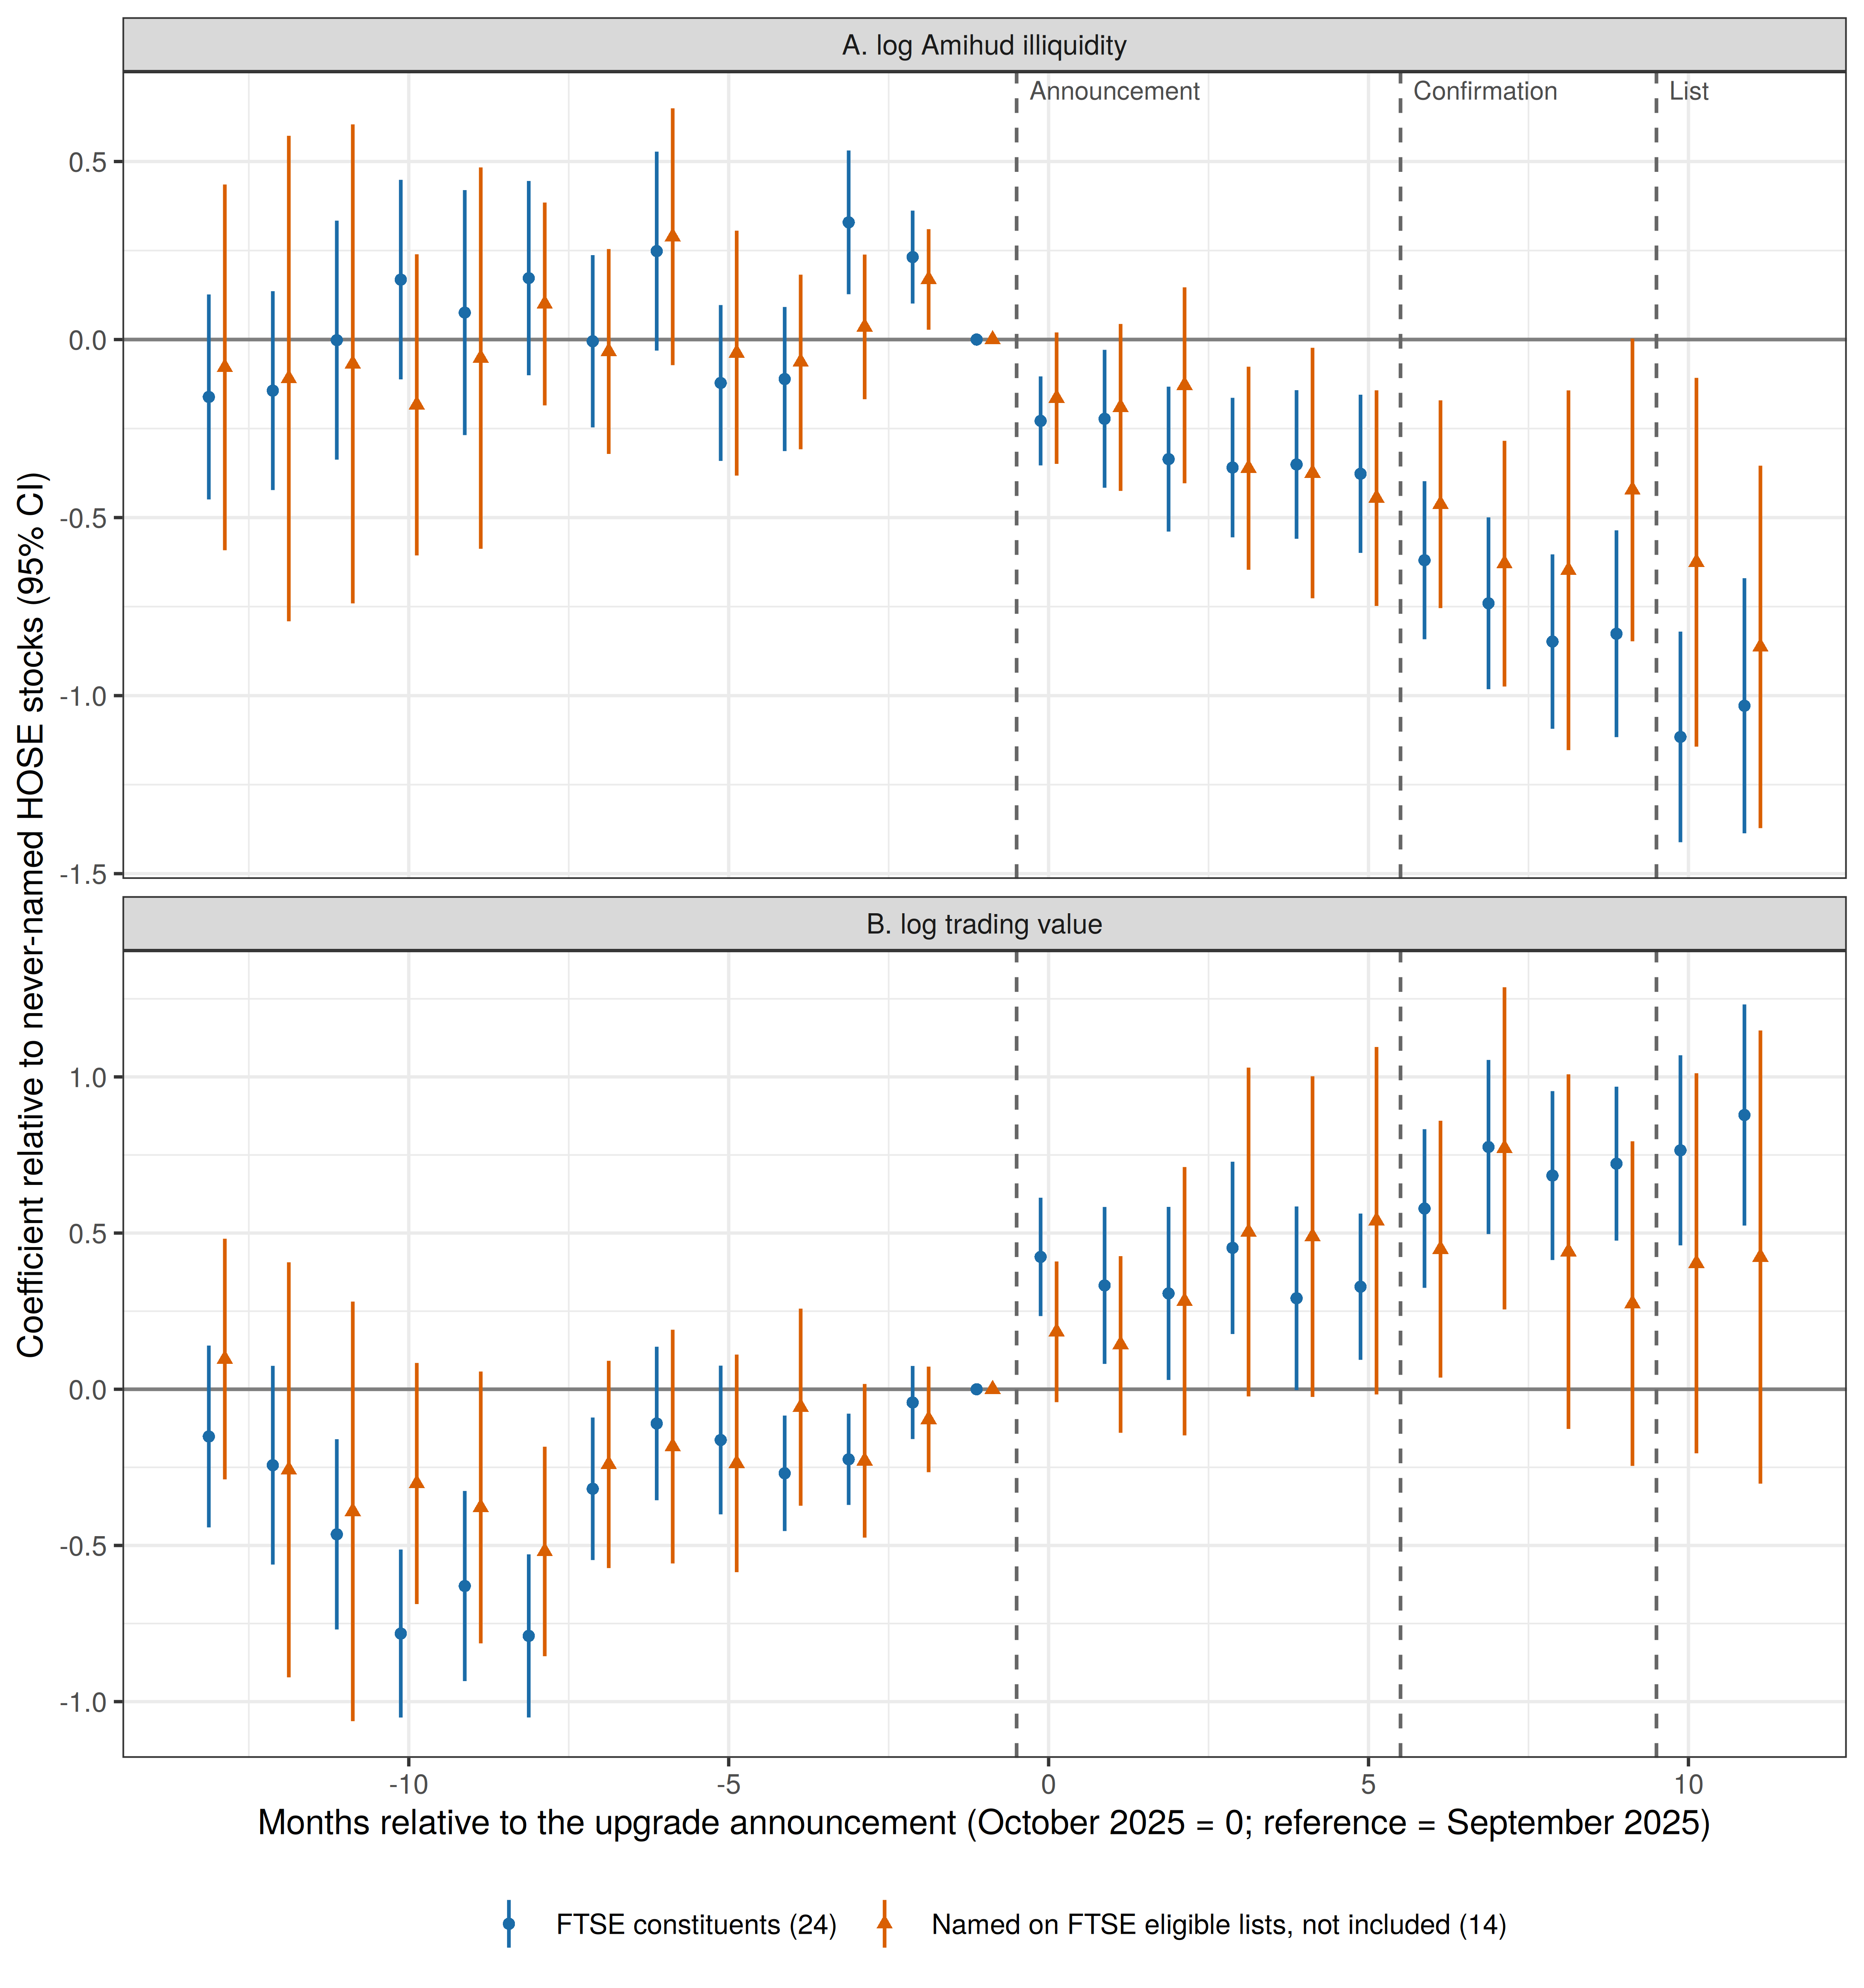
\includegraphics[width=0.95\textwidth]{Figure_1.png}\par\medskip
{\small \emph{Note}: Coefficients \(\delta_m\) of Eq. (8) with 95\% confidence
intervals (panel A: log Amihud; panel B: log trading value); dashed
lines mark the announcement, confirmation and list months. Source:
Authors' calculations.}
\end{figure}

\begin{figure}[p]
\noindent \textbf{Figure 2. Monthly event-study coefficients for the
intention-to-treat group}\par\medskip
\noindent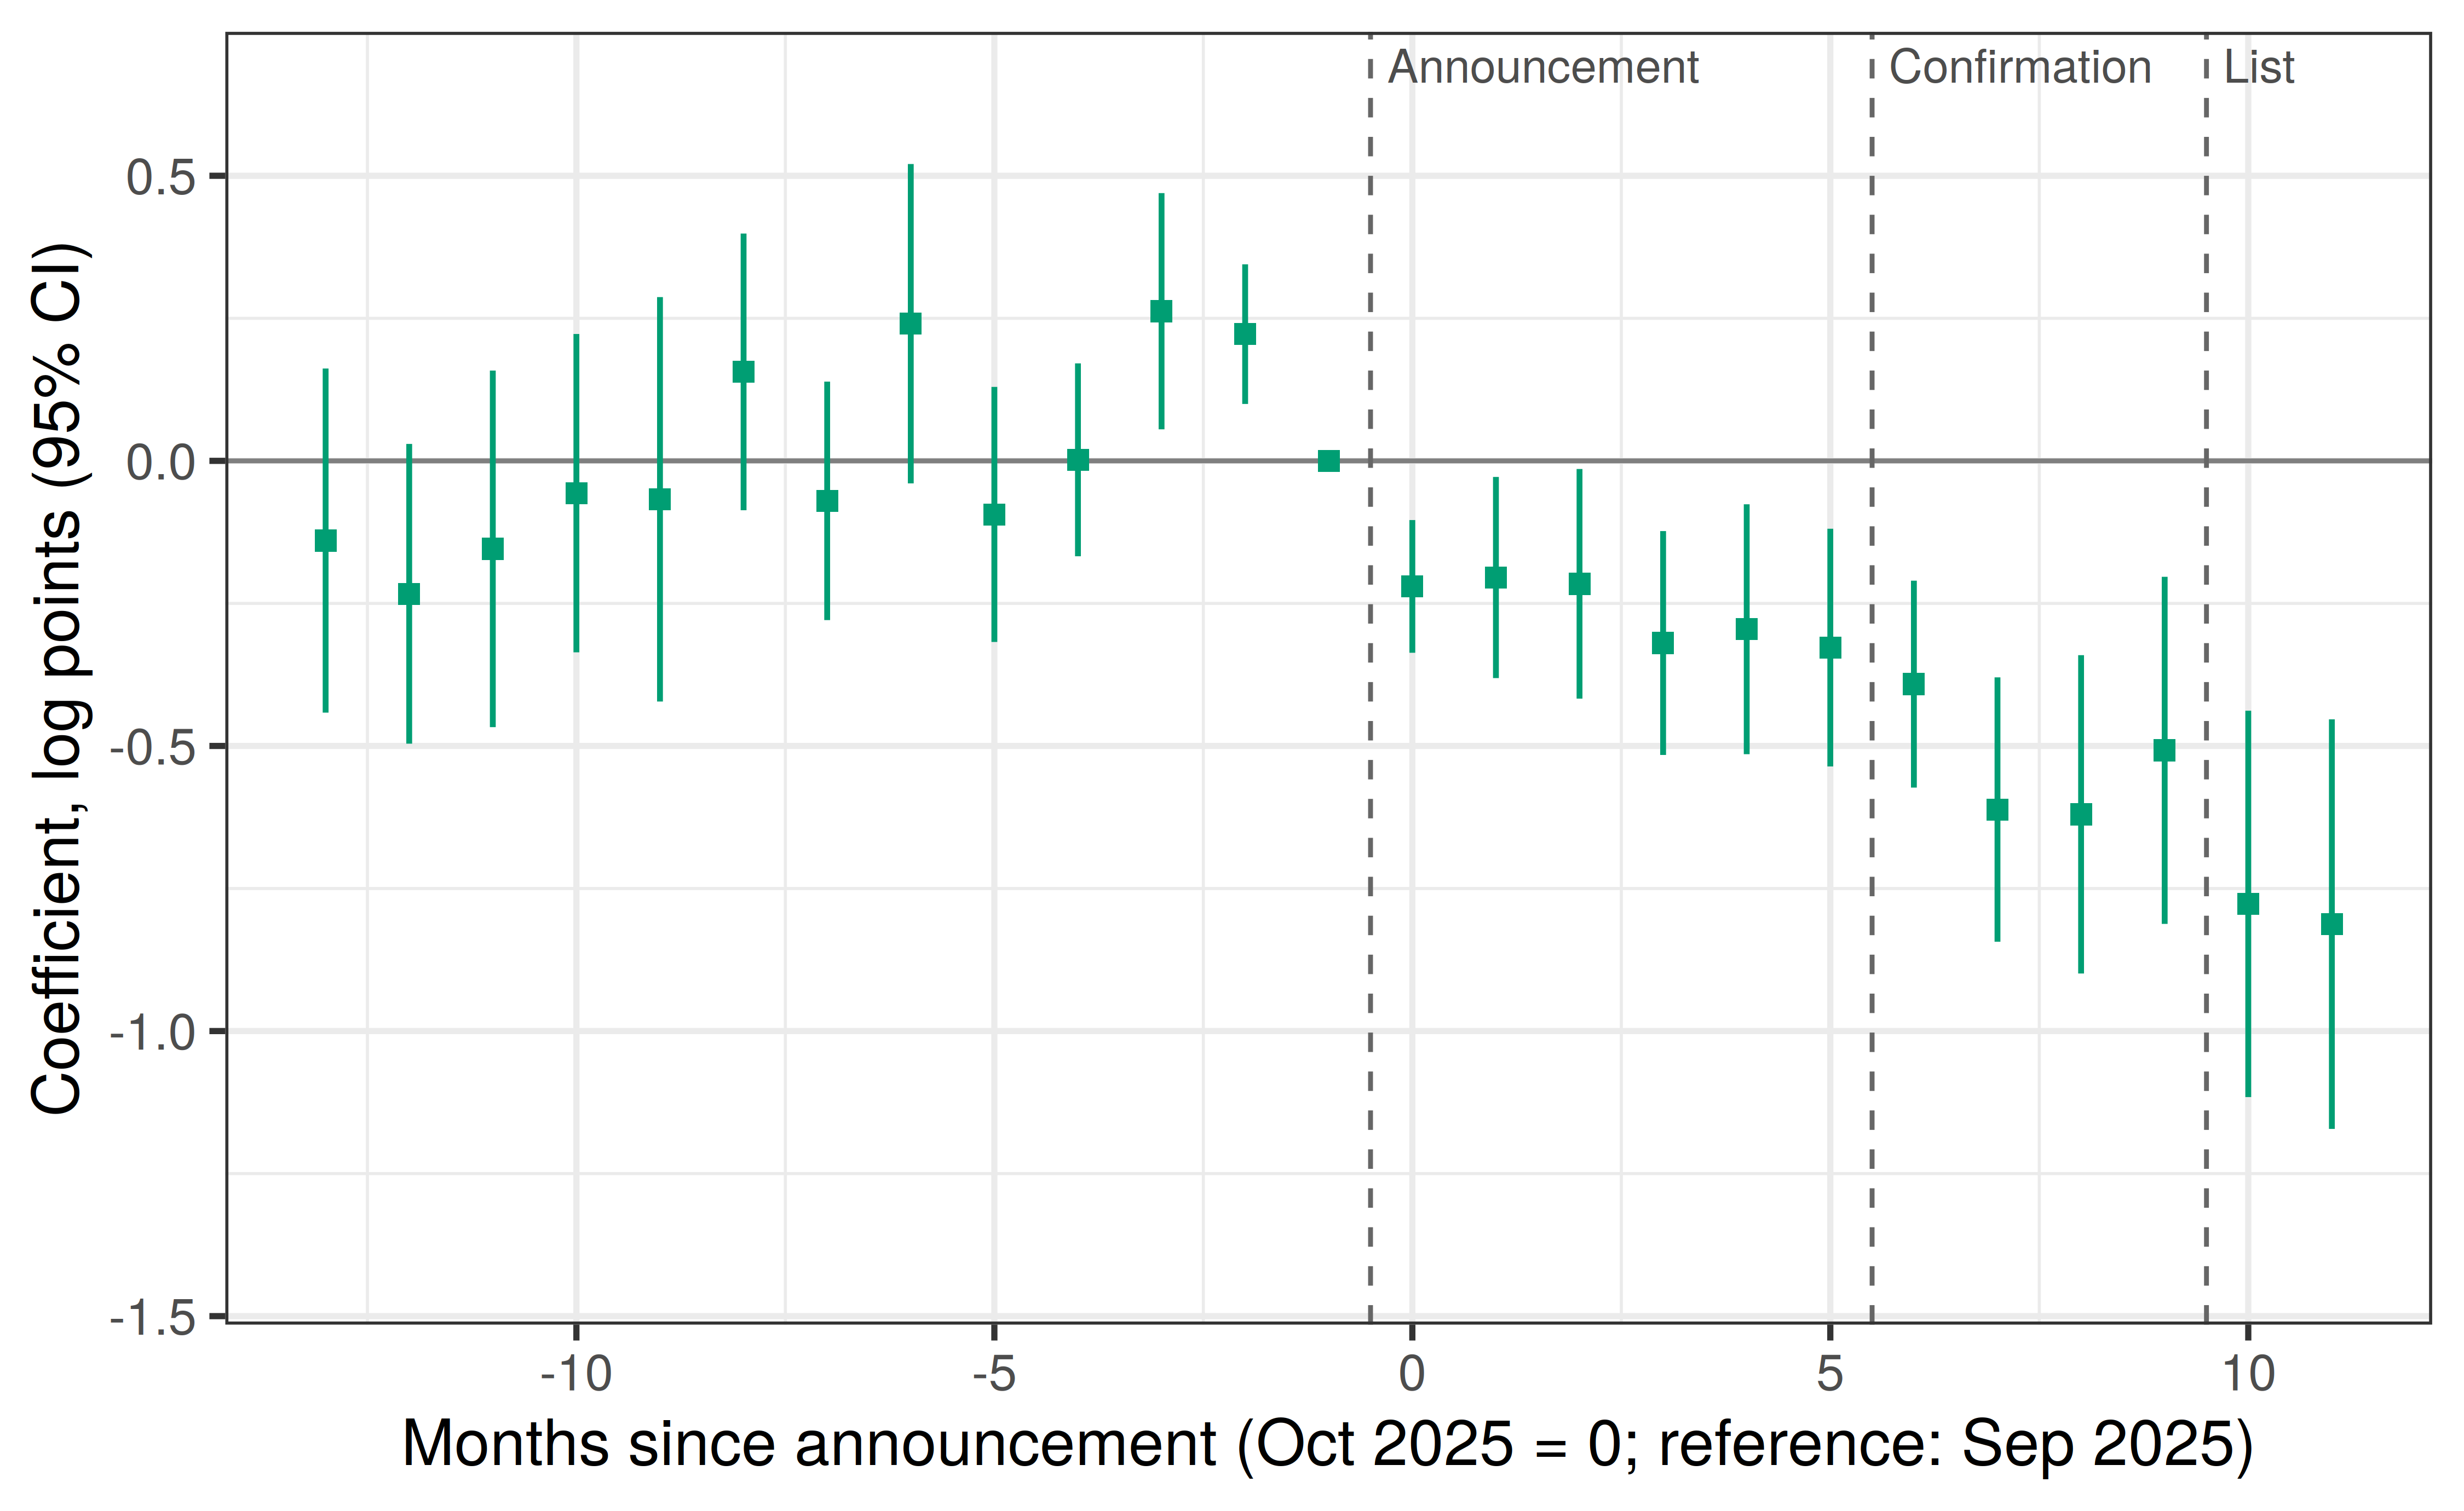
\includegraphics[width=0.95\textwidth]{Figure_2.png}\par\medskip
{\small \emph{Note}: Eq. (8) for log Amihud with \(\mathrm{ITT}_i\) in place of
\(\mathrm{Constituent}_i\) and 95\% confidence intervals; dashed lines
as in Figure 1. Source: Authors' calculations.}
\end{figure}

The trading value of constituents rose by 0.68, 1.03 and 1.19 log points
(Table 2, column 2) but was already rising before October 2025 (Figure
1, panel B); given the trend-adjusted estimates in Section 5.1, we
describe the trading-value result as an association.

Randomization inference confirms that the declines exceed those of large
HOSE stocks in general: none of 500 pseudo-groups of 24 stocks drawn
from the 85 largest never-named stocks produced a coefficient as
negative as the observed one in any window (one-sided \emph{p}
\textless{} 0.002). The placebo distribution centres at −0.21 in the
list window, less than one fifth of the constituent effect.

\hypertarget{prices-moved-at-the-announcement-and-the-confirmation}{%
\subsection*{4.2 Prices moved at the announcement and the
confirmation}}

Table 4 reports CARs with portfolio \emph{t}-statistics for every
pre-specified window. Over days −1 to +5 around the announcement,
constituents earned 3.9\% to 7.8\% depending on the benchmark (\emph{t}
between 2.19 and 3.46), and over days −1 to +1 around the confirmation,
2.7\% to 4.5\% (\emph{t} between 2.22 and 2.93); these are the only
reliable disclosure-window CARs. The three-day announcement CAR is
significant under one benchmark only, so the response built up over the
week. Around the constituent list, the three-day CARs (1.5\% to 2.7\%)
are never significant and the {[}−1,+5{]} CARs (2.0\% to 4.4\%) are
significant under two benchmarks. The data end two sessions after the
effective date, so only its {[}−1,+1{]} window exists; that CAR (−0.5\%
to 0.9\%) is never significant. Cross-sectional \emph{t}-statistics,
which ignore the common event date, are up to 2.9 times larger (6.48
against 2.27 for the three-day announcement CAR). The announcement-week
response parallels the short-term excess returns that Dong et al.~(2023)
report around the announcement of the China A-share inclusion.

\needspace{14\baselineskip}\textbf{Table 4. Cumulative abnormal returns around FTSE disclosures}

Panel A. Constituents (24)

\begin{longtable}[]{@{}>{\raggedright\arraybackslash}p{(\linewidth - 10\tabcolsep) * \real{0.2600}}>{\raggedright\arraybackslash}p{(\linewidth - 10\tabcolsep) * \real{0.1480}}>{\raggedright\arraybackslash}p{(\linewidth - 10\tabcolsep) * \real{0.1480}}>{\raggedright\arraybackslash}p{(\linewidth - 10\tabcolsep) * \real{0.1480}}>{\raggedright\arraybackslash}p{(\linewidth - 10\tabcolsep) * \real{0.1480}}>{\raggedright\arraybackslash}p{(\linewidth - 10\tabcolsep) * \real{0.1480}}@{}}
\toprule\noalign{}
\begin{minipage}[b]{\linewidth}\raggedright
Event
\end{minipage} & \begin{minipage}[b]{\linewidth}\centering
Window
\end{minipage} & \begin{minipage}[b]{\linewidth}\centering
Never-named
\end{minipage} & \begin{minipage}[b]{\linewidth}\centering
Matched
\end{minipage} & \begin{minipage}[b]{\linewidth}\centering
Large never-named
\end{minipage} & \begin{minipage}[b]{\linewidth}\centering
Market model
\end{minipage} \\
\midrule\noalign{}
\endhead
\bottomrule\noalign{}
\endlastfoot
Announcement (7 Oct 2025) & {[}−1,+1{]} & 3.3\% (2.27) & 1.7\% (1.43) &
2.3\% (1.54) & 2.6\% (1.85) \\
& {[}−1,+5{]} & 7.8\% (3.46) & 3.9\% (2.19) & 6.3\% (2.75) & 6.6\%
(3.04) \\
& {[}0,+20{]} & −2.4\% (−0.61) & 1.6\% (0.51) & −1.4\% (−0.35) & −5.5\%
(−1.47) \\
Confirmation (7 Apr 2026) & {[}−1,+1{]} & 4.5\% (2.93) & 2.7\% (2.22) &
3.6\% (2.73) & 3.8\% (2.73) \\
& {[}−1,+5{]} & 4.7\% (2.00) & 2.2\% (1.21) & 3.5\% (1.75) & 3.6\%
(1.72) \\
& {[}0,+20{]} & 10.0\% (2.44) & 6.2\% (1.94) & 10.6\% (3.03) & 8.4\%
(2.30) \\
Constituent list (21 Aug 2026) & {[}−1,+1{]} & 2.7\% (1.86) & 1.5\%
(1.31) & 1.8\% (1.50) & 1.5\% (1.25) \\
& {[}−1,+5{]} & 4.4\% (2.04) & 2.0\% (1.12) & 3.9\% (2.17) & 3.1\%
(1.64) \\
& {[}0,+20{]} & 4.6\% (1.21) & 3.7\% (1.21) & 5.2\% (1.65) & 3.3\%
(1.00) \\
Effective date (21 Sep 2026) & {[}−1,+1{]} & −0.1\% (−0.11) & 0.9\%
(0.88) & 0.0\% (0.03) & −0.5\% (−0.51) \\
\end{longtable}

Panel B. ITT group (27)

\begin{longtable}[]{@{}>{\raggedright\arraybackslash}p{(\linewidth - 10\tabcolsep) * \real{0.2600}}>{\raggedright\arraybackslash}p{(\linewidth - 10\tabcolsep) * \real{0.1480}}>{\raggedright\arraybackslash}p{(\linewidth - 10\tabcolsep) * \real{0.1480}}>{\raggedright\arraybackslash}p{(\linewidth - 10\tabcolsep) * \real{0.1480}}>{\raggedright\arraybackslash}p{(\linewidth - 10\tabcolsep) * \real{0.1480}}>{\raggedright\arraybackslash}p{(\linewidth - 10\tabcolsep) * \real{0.1480}}@{}}
\toprule\noalign{}
\begin{minipage}[b]{\linewidth}\raggedright
Event
\end{minipage} & \begin{minipage}[b]{\linewidth}\centering
Window
\end{minipage} & \begin{minipage}[b]{\linewidth}\centering
Never-named
\end{minipage} & \begin{minipage}[b]{\linewidth}\centering
Matched
\end{minipage} & \begin{minipage}[b]{\linewidth}\centering
Large never-named
\end{minipage} & \begin{minipage}[b]{\linewidth}\centering
Market model
\end{minipage} \\
\midrule\noalign{}
\endhead
\bottomrule\noalign{}
\endlastfoot
Announcement (7 Oct 2025) & {[}−1,+1{]} & 3.0\% (2.43) & 1.3\% (1.07) &
2.0\% (1.87) & 2.3\% (2.05) \\
& {[}−1,+5{]} & 7.5\% (3.97) & 3.5\% (1.91) & 5.9\% (3.72) & 6.4\%
(3.75) \\
& {[}0,+20{]} & −1.0\% (−0.32) & 2.9\% (0.90) & −0.1\% (−0.03) & −3.6\%
(−1.20) \\
Confirmation (7 Apr 2026) & {[}−1,+1{]} & 3.1\% (2.17) & 1.3\% (0.99) &
2.2\% (2.10) & 2.4\% (2.02) \\
& {[}−1,+5{]} & 3.2\% (1.45) & 0.7\% (0.35) & 2.0\% (1.24) & 2.3\%
(1.25) \\
& {[}0,+20{]} & 7.0\% (1.83) & 3.2\% (0.94) & 7.6\% (2.74) & 6.3\%
(2.01) \\
Constituent list (21 Aug 2026) & {[}−1,+1{]} & 2.7\% (2.08) & 1.6\%
(1.37) & 1.8\% (2.13) & 1.7\% (1.64) \\
& {[}−1,+5{]} & 3.2\% (1.62) & 0.7\% (0.42) & 2.7\% (2.05) & 2.3\%
(1.43) \\
& {[}0,+20{]} & 1.2\% (0.35) & 0.3\% (0.11) & 1.8\% (0.80) & 1.4\%
(0.50) \\
Effective date (21 Sep 2026) & {[}−1,+1{]} & 0.4\% (0.35) & 1.5\% (1.52)
& 0.6\% (0.75) & 0.2\% (0.27) \\
\end{longtable}

\emph{Notes}: CARs in percent from Eq. (6), for windows in trading days
around each disclosure, with portfolio \emph{t}-statistics in
parentheses and the benchmarks of Section 3.2. Source: Authors'
calculations.

The two gains behaved differently afterwards. Over days 0 to +20 the
announcement CAR lies between −5.5\% and 1.6\% and is never significant,
whereas after the confirmation constituents earned 6.2\% to 10.6\%,
significant under three of four benchmarks (\emph{t} between 1.94 and
3.03). The fading after the conditional announcement is consistent with
temporary price pressure: in Harris and Gurel (1986), S\&P 500 additions
gained more than 3\% on the announcement, and the gain was almost fully
reversed after two weeks. The lasting gain after the confirmation, once
the upgrade was certain and dated, is consistent with a shift in demand
(Shleifer, 1986; Chen et al., 2004) and with the persistent gains of
frontier-market index additions (Biktimirov \& Afego, 2026). Our data
end too soon to test for the reversal within a year that Burnham et
al.~(2018) find at the country level.

Panel B reports the ITT group, and we add the named-but-excluded stocks
in the text. The ITT group earned 3.5\% to 7.5\% in the announcement
week, significant under three of four benchmarks (the matched benchmark
yields \emph{t} = 1.91), and 1.3\% to 3.1\% over three days at the
confirmation, significant except against matched controls.
Named-but-excluded stocks gained 2.3\% to 6.2\% in the announcement week
(significant under three of four benchmarks) and nothing at the
confirmation (−1.4\% to 0.4\%, never significant; not tabulated). No
list was public at the announcement, so their announcement-week gain
suggests that investors responded to characteristics they could observe,
such as size and liquidity. By the confirmation the preliminary list was
public, and only stocks that went on to be included gained. These
results support H3 for the announcement and the confirmation but not for
the constituent list.

\hypertarget{the-rebalancing-session-produced-a-trading-surge-only-for-included-stocks}{%
\subsection*{4.3 The rebalancing session produced a trading surge only
for included
stocks}}

In Table 5 (Eq. 9), the log trading value of constituents on 18
September 2026, the last session before the upgrade took effect, rose
0.79 above its level on other sessions in the window, relative to
never-named stocks (standard error 0.12, \emph{t} = 6.84), and 0.84
relative to matched controls. On the effective date the excess fell to
0.20 (\emph{p} = 0.057) and 0.34 (\emph{p} = 0.007). Named-but-excluded
stocks show no surge (−0.01 and −0.16). Mean abnormal log trading value
on 18 September was 0.76 for constituents (standard error 0.12), −0.28
for matched controls (0.10) and 0.00 for named-but-excluded stocks
(0.15).

\needspace{14\baselineskip}\textbf{Table 5. Excess log trading value on the rebalancing and
effective sessions}

\begin{longtable}[]{@{}>{\raggedright\arraybackslash}p{(\linewidth - 6\tabcolsep) * \real{0.3400}}>{\raggedright\arraybackslash}p{(\linewidth - 6\tabcolsep) * \real{0.2200}}>{\raggedright\arraybackslash}p{(\linewidth - 6\tabcolsep) * \real{0.2200}}>{\raggedright\arraybackslash}p{(\linewidth - 6\tabcolsep) * \real{0.2200}}@{}}
\toprule\noalign{}
\begin{minipage}[b]{\linewidth}\raggedright
Comparison
\end{minipage} & \begin{minipage}[b]{\linewidth}\centering
18 Sep 2026 (rebalancing)
\end{minipage} & \begin{minipage}[b]{\linewidth}\centering
21 Sep 2026 (effective date)
\end{minipage} & \begin{minipage}[b]{\linewidth}\centering
Observations
\end{minipage} \\
\midrule\noalign{}
\endhead
\bottomrule\noalign{}
\endlastfoot
Constituents vs never-named & 0.794*** (0.116) & 0.202 (0.106) &
10,820 \\
Constituents vs matched controls & 0.837*** (0.122) & 0.341** (0.122) &
1,536 \\
Named-but-excluded vs never-named & −0.013 (0.116) & −0.159 (0.136) &
10,500 \\
\end{longtable}

\emph{Notes}: Eq. (9) over 6 August to 23 September 2026; other details
as in Table 2. Source: Authors' calculations.

The surge matches the trading that funds tracking FTSE benchmarks had to
do: they were to buy the first tranche at the closing price of 18
September (FTSE Russell, 2026; VIR, 2026), and nothing obliged them to
trade the stocks FTSE had passed over. Without data on who traded, we
infer index demand from the timing and from the missing surge for
named-but-excluded stocks, where a general rise in trading would have
shown up. Prices showed no reliable change: the three-day CAR around the
effective date lies between −0.5\% and 0.9\% (Table 4), consistent with
other investors having bought earlier and supplying the stocks at the
close, and with the second half of H3. Harris and Gurel (1986), by
contrast, find price rises immediately after S\&P 500 additions are
announced, which they attribute to index-fund buying pressure. The
illiquidity decline at the disclosures and the volume surge at the close
are consistent with the two stages at which benchmark changes move fund
allocations, announcement and implementation (Raddatz et al., 2017).

\hypertarget{the-rebalancing-surge-rose-with-ftse-size-segment}{%
\subsection*{4.4 The rebalancing surge rose with FTSE size
segment}}

FTSE assigned the constituents to size segments on 21 August 2026: three
large-capitalization stocks (VCB, VIC, VHM), three mid-capitalization
stocks (BID, VPB, HPG) and 18 small-capitalization stocks in our sample
(VIR, 2026). H4 predicts a larger rebalancing surge for large
constituents, whose index weights are larger, and benchmark-driven
foreign allocations (Raddatz et al., 2017) suggest the same ordering for
the persistent liquidity effect.

Table 6 splits the constituent coefficients by segment. Illiquidity fell
most for the three large stocks (−0.61, −1.35 and −2.20 log points),
against −0.20, −0.63 and −0.82 for mid and −0.39, −0.85 and −1.00 for
small stocks. The mid-small ordering does not follow size, and with
three stocks in each upper segment we read these estimates as
descriptive. The rebalancing surge rose monotonically with segment
(abnormal log trading value of 1.23, 0.98 and 0.65), consistent with H4,
although the two upper segments contain three stocks each.

\needspace{14\baselineskip}\textbf{Table 6. Constituent effects by FTSE size segment}

\begin{longtable}[]{@{}>{\raggedright\arraybackslash}p{(\linewidth - 6\tabcolsep) * \real{0.3400}}>{\raggedright\arraybackslash}p{(\linewidth - 6\tabcolsep) * \real{0.2200}}>{\raggedright\arraybackslash}p{(\linewidth - 6\tabcolsep) * \real{0.2200}}>{\raggedright\arraybackslash}p{(\linewidth - 6\tabcolsep) * \real{0.2200}}@{}}
\toprule\noalign{}
\begin{minipage}[b]{\linewidth}\raggedright
Outcome, window
\end{minipage} & \begin{minipage}[b]{\linewidth}\centering
Large (3)
\end{minipage} & \begin{minipage}[b]{\linewidth}\centering
Mid (3)
\end{minipage} & \begin{minipage}[b]{\linewidth}\centering
Small (18)
\end{minipage} \\
\midrule\noalign{}
\endhead
\bottomrule\noalign{}
\endlastfoot
Amihud, announcement & −0.607 (0.273) & −0.204 (0.119) & −0.387***
(0.113) \\
Amihud, confirmation & −1.350 (0.413) & −0.629 (0.076) & −0.855***
(0.133) \\
Amihud, list & −2.198 (0.396) & −0.819 (0.229) & −1.002*** (0.187) \\
Trading value, list & 2.332 (0.484) & 0.896 (0.194) & 1.048***
(0.160) \\
Abnormal trading value, 18 Sep & 1.231 (0.110) & 0.976 (0.294) & 0.645
(0.150) \\
\end{longtable}

\emph{Notes}: Eq. (7) with segment-by-window interactions; the last row
reports the mean (standard error), and significance marks are omitted
for the three-stock segments. Source: Authors' calculations.

\hypertarget{volatility-rose-so-the-illiquidity-decline-is-conservative}{%
\subsection*{4.5 Volatility rose, so the illiquidity decline is
conservative}}

In Table 7, the weekly volatility of constituents rose by 0.34 and 0.21
log points in the announcement and confirmation windows (both
significant at 0.1\%) and by an insignificant 0.14 in the list window
(column 1). Because the Amihud ratio divides absolute returns by traded
value (Amihud, 2002), rising volatility pushes it up, so the measured
decline in illiquidity understates the gain in trading capacity.
Controlling for volatility enlarges the Amihud coefficients to −0.57,
−1.00 and −1.20 (column 5).

The CS spread rose by 0.09 to 0.13 percentage points (column 2), and by
0.11 to 0.14 percentage points in the matched sample (column 3), from a
pre-period mean of 0.57\%; with the volatility control, the rise shrinks
to 0.06, 0.08 and 0.12 percentage points (column 4). The rise contrasts
with S\&P 500 additions, whose liquidity gain came mainly through lower
direct trading costs (Hegde \& McDermott, 2003). Because the Corwin and
Schultz (2012) estimator loads on intraday price ranges, the residual
rise may reflect volatility the weekly control misses, so we limit our
liquidity claims to price impact and trading activity.

\needspace{14\baselineskip}\textbf{Table 7. Volatility, CS spread and Amihud estimates for
constituents}

\begin{longtable}[]{@{}>{\raggedright\arraybackslash}p{(\linewidth - 10\tabcolsep) * \real{0.2600}}>{\raggedright\arraybackslash}p{(\linewidth - 10\tabcolsep) * \real{0.1480}}>{\raggedright\arraybackslash}p{(\linewidth - 10\tabcolsep) * \real{0.1480}}>{\raggedright\arraybackslash}p{(\linewidth - 10\tabcolsep) * \real{0.1480}}>{\raggedright\arraybackslash}p{(\linewidth - 10\tabcolsep) * \real{0.1480}}>{\raggedright\arraybackslash}p{(\linewidth - 10\tabcolsep) * \real{0.1480}}@{}}
\toprule\noalign{}
\begin{minipage}[b]{\linewidth}\raggedright
Window
\end{minipage} & \begin{minipage}[b]{\linewidth}\centering
(1) Volatility
\end{minipage} & \begin{minipage}[b]{\linewidth}\centering
(2) CS spread
\end{minipage} & \begin{minipage}[b]{\linewidth}\centering
(3) CS spread, matched
\end{minipage} & \begin{minipage}[b]{\linewidth}\centering
(4) CS spread, volatility control
\end{minipage} & \begin{minipage}[b]{\linewidth}\centering
(5) Amihud, volatility control
\end{minipage} \\
\midrule\noalign{}
\endhead
\bottomrule\noalign{}
\endlastfoot
Announcement & 0.341*** (0.058) & 0.0009** (0.0003) & 0.0011** (0.0004)
& 0.0006* (0.0003) & −0.574*** (0.102) \\
Confirmation & 0.215*** (0.056) & 0.0010** (0.0003) & 0.0014*** (0.0004)
& 0.0008* (0.0003) & −1.003*** (0.122) \\
List & 0.139 (0.086) & 0.0013** (0.0005) & 0.0013* (0.0006) & 0.0012*
(0.0005) & −1.203*** (0.164) \\
Volatility & & & & 0.0010*** (0.0001) & 0.535*** (0.021) \\
Observations & 34,369 & 34,369 & 4,751 & 34,369 & 34,369 \\
\end{longtable}

\emph{Notes}: Eq. (7), with volatility \(\mathrm{Vol}_{iw}\) from Eq.
(4) and spreads in decimal units (0.0010 = 0.10 percentage points).
Source: Authors' calculations.

\hypertarget{robustness-and-selection}{%
\section*{5. Robustness and selection}}

\hypertarget{robustness-of-the-liquidity-result}{%
\subsection*{5.1 Robustness of the liquidity
result}}

Table 8 collects the robustness checks for the constituent Amihud
result. The coefficients remain negative in every specification; they
are of similar size except in the weighted matched sample with a trend
and the drift specification, where they are about half as large (the ITT
row compares with Table 3).

\needspace{14\baselineskip}\textbf{Table 8. Robustness of the constituent Amihud estimates}

\begin{longtable}[]{@{}>{\raggedright\arraybackslash}p{(\linewidth - 8\tabcolsep) * \real{0.2600}}>{\raggedright\arraybackslash}p{(\linewidth - 8\tabcolsep) * \real{0.1850}}>{\raggedright\arraybackslash}p{(\linewidth - 8\tabcolsep) * \real{0.1850}}>{\raggedright\arraybackslash}p{(\linewidth - 8\tabcolsep) * \real{0.1850}}>{\raggedright\arraybackslash}p{(\linewidth - 8\tabcolsep) * \real{0.1850}}@{}}
\toprule\noalign{}
\begin{minipage}[b]{\linewidth}\raggedright
Specification
\end{minipage} & \begin{minipage}[b]{\linewidth}\centering
Announcement
\end{minipage} & \begin{minipage}[b]{\linewidth}\centering
Confirmation
\end{minipage} & \begin{minipage}[b]{\linewidth}\centering
List
\end{minipage} & \begin{minipage}[b]{\linewidth}\centering
Observations
\end{minipage} \\
\midrule\noalign{}
\endhead
\bottomrule\noalign{}
\endlastfoot
Baseline (Table 2, column 1) & −0.392*** (0.098) & −0.888*** (0.124) &
−1.129*** (0.178) & 34,369 \\
Size-tercile-by-week fixed effects & −0.424*** (0.108) & −0.786***
(0.139) & −0.978*** (0.207) & 34,369 \\
Excl. Vingroup stocks & −0.389*** (0.100) & −0.863*** (0.114) &
−1.007*** (0.168) & 34,072 \\
Linear trend & −0.382*** (0.098) & −0.874*** (0.156) & −1.111*** (0.225)
& 34,369 \\
Matched sample with trend & −0.204 (0.138) & −0.425* (0.199) & −0.637*
(0.262) & 4,751 \\
Post-announcement drift & −0.231* (0.110) & −0.446** (0.171) & −0.541*
(0.235) & 34,369 \\
Excl. July and August 2025 & −0.354*** (0.105) & −0.850*** (0.130) &
−1.091*** (0.183) & 31,212 \\
Excl. banks and brokers (11) & −0.439** (0.163) & −1.042*** (0.210) &
−1.398*** (0.315) & 33,082 \\
ITT excl. banks and brokers (19) & −0.225* (0.095) & −0.515** (0.163) &
−0.831*** (0.223) & 33,874 \\
Wild cluster bootstrap \emph{p} & \textless{} 0.001 & \textless{} 0.001
& \textless{} 0.001 & \\
Randomization inference \emph{p} & \textless{} 0.002 & \textless{} 0.002
& \textless{} 0.002 & \\
\end{longtable}

\emph{Notes}: Dependent variable log Amihud; the excluded stocks and the
inference settings are given in Sections 3.3 and 5.1. Source: Authors'
calculations.

\textbf{Pre-announcement months.} The positive pre-period deviations in
Figure 1 work against the estimated declines. Dropping July and August
2025, the two months with significant positive deviations, or adding a
constituent-specific linear trend (−0.0002 per week, standard error
0.003) leaves the estimates almost unchanged (Table 8). The weighted
matched sample with a trend yields estimates about half as large, with
the announcement estimate not significant, so we rest the
announcement-stage conclusion on the full-sample, ITT and trend
estimates and treat it as less certain than the later stages.

\textbf{Size-related shocks.} With size-tercile-by-week fixed effects,
the confirmation and list coefficients shrink by 12\% and 13\% and all
three remain significant at 0.1\%; the predicted-constituent estimates
in Table 3, which use only pre-period size, point the same way.

\textbf{Trading value.} A constituent-specific linear trend in trading
value is strong (0.010 log points per week, \emph{p} \textless{} 0.001),
and trend-adjusted effects fall to 0.28, 0.39 and 0.43 log points, the
last significant only at 10\%.

\textbf{Inference and influential stocks.} Two-way clustering by stock
and week widens standard errors by less than 17\%. Excluding the three
Vingroup-family stocks changes the estimates by at most 11\%. In the
unweighted matched sample, with 48 clusters, the wild cluster bootstrap
\emph{p}-values remain at or below 0.003.

\textbf{Sector composition and the pre-funding reform.} Banks (VCB, BID,
VPB, HDB, STB, SHB, SSB, MSB) and securities firms (SSI, VCI, VIX, VND,
HCM) make up 13 of the 24 constituents and 8 of the 27 ITT stocks, which
also include EIB; the Vingroup stocks are VIC, VHM and VRE. Without the
banks and securities firms, the remaining 11 constituents and 19 ITT
stocks show similar or larger declines (Table 8). LSEG (2026) lists the
removal of pre-funding requirements for foreign institutional investors
among the reforms behind the upgrade, a reform that applies to every
stock foreign investors can buy. The 85 large never-named stocks also
became more liquid (Section 4.1), but this comparison does not separate
the reform from the upgrade for the largest stocks.

\textbf{Placebo.} A fake event on 7 April 2025, estimated on
pre-announcement data only, yields a coefficient of 0.04 (standard error
0.10).

\hypertarget{selection-ftses-lists-partly-followed-rising-liquidity}{%
\subsection*{5.2 Selection: FTSE's lists partly followed rising
liquidity}}

Table 9 uses the 14 stocks FTSE named but did not include to test for
selection. They became less illiquid than never-named stocks by 0.29,
0.55 and 0.87 log points, 62\% to 77\% of the constituent effects, the
first significant only at 10\% (panel A). Without BSR, whose pre-period
spans two venues, the estimates are −0.23, −0.46 and −0.73, only the
last significant at 5\%. The gains concentrate in GEE and BSR.

Panel B splits the period after the announcement into three screening
windows, assigning weeks by their start date: S1 from 7 October to 31
December 2025, the last date of the data FTSE screened for the April
2026 list; S2 from 1 January to 6 April 2026; and S3 from 7 April 2026.
GEE, added in April, became 1.83 log points less illiquid relative to
never-named stocks during S1, inside that data window (Appendix Table
A.3). BSR improved mostly after the cut-off (−0.39 in S1, −1.68 in S2).
It joined HOSE only in January 2025, after the data date of the November
list (VietnamPlus, 2024), which provides a reason other than liquidity
for its later addition. The twelve November names changed little (−0.02,
−0.19 and −0.30 log points, none significant at 5\%), and only PLX,
which FTSE dropped in April, and DPM fell by more than 0.5 log points by
the April list.

\needspace{14\baselineskip}\textbf{Table 9. Named-but-excluded stocks and the timing of FTSE's
screening}

Panel A. Named-but-excluded (14) and constituents

\begin{longtable}[]{@{}>{\raggedright\arraybackslash}p{(\linewidth - 6\tabcolsep) * \real{0.3400}}>{\raggedright\arraybackslash}p{(\linewidth - 6\tabcolsep) * \real{0.2200}}>{\raggedright\arraybackslash}p{(\linewidth - 6\tabcolsep) * \real{0.2200}}>{\raggedright\arraybackslash}p{(\linewidth - 6\tabcolsep) * \real{0.2200}}@{}}
\toprule\noalign{}
\begin{minipage}[b]{\linewidth}\raggedright
Window
\end{minipage} & \begin{minipage}[b]{\linewidth}\centering
Constituents: Amihud
\end{minipage} & \begin{minipage}[b]{\linewidth}\centering
Named: Amihud
\end{minipage} & \begin{minipage}[b]{\linewidth}\centering
Named: trading value
\end{minipage} \\
\midrule\noalign{}
\endhead
\bottomrule\noalign{}
\endlastfoot
Announcement & −0.392*** (0.098) & −0.293 (0.154) & 0.589** (0.186) \\
Confirmation & −0.888*** (0.124) & −0.554* (0.255) & 0.683* (0.269) \\
List and rebalancing & −1.129*** (0.178) & −0.865** (0.304) & 0.653
(0.345) \\
\end{longtable}

Panel B. log Amihud by screening window

\begin{longtable}[]{@{}>{\raggedright\arraybackslash}p{(\linewidth - 6\tabcolsep) * \real{0.3400}}>{\raggedright\arraybackslash}p{(\linewidth - 6\tabcolsep) * \real{0.2200}}>{\raggedright\arraybackslash}p{(\linewidth - 6\tabcolsep) * \real{0.2200}}>{\raggedright\arraybackslash}p{(\linewidth - 6\tabcolsep) * \real{0.2200}}@{}}
\toprule\noalign{}
\begin{minipage}[b]{\linewidth}\raggedright
Group
\end{minipage} & \begin{minipage}[b]{\linewidth}\centering
S1
\end{minipage} & \begin{minipage}[b]{\linewidth}\centering
S2
\end{minipage} & \begin{minipage}[b]{\linewidth}\centering
S3
\end{minipage} \\
\midrule\noalign{}
\endhead
\bottomrule\noalign{}
\endlastfoot
Constituents (24) & −0.339** (0.110) & −0.440*** (0.100) & −0.932***
(0.129) \\
Named Nov 2025, not included (12) & −0.024 (0.092) & −0.185 (0.127) &
−0.295 (0.168) \\
Added Apr 2026: GEE, BSR & −1.15 & −1.67 & −2.51 \\
\end{longtable}

\emph{Notes}: One regression per panel on all 366 stocks, relative to
never-named stocks, with point estimates only for the two-stock row;
other details as in Table 2. Source: Authors' calculations.

FTSE's screens rest on investability, and at least one stock became
eligible after its liquidity rose during the screening window. The same
can happen among the final constituents, chosen on June 2026 data, and
could favour stocks with large gains on disclosure dates. Studies that
use index additions as an exogenous liquidity shock (Becker-Blease \&
Paul, 2006) rely on membership not following liquidity; the Vietnamese
lists show that this premise can fail when the index provider screens on
recent liquidity. The ITT group, fixed on 2024 data, is not exposed to
this selection and still shows illiquidity declines of 24\% to 56\% and
an announcement-week price response significant under three of four
benchmarks. We report both sets of estimates and treat neither as a
bound on the other.

\hypertarget{discussion-and-conclusion}{%
\section*{6. Discussion and conclusion}}

Liquidity and price gains for likely index stocks came with FTSE's
disclosures of Vietnam's reclassification, before the first index
tranche took effect. The pre-announcement eligible stocks became 24\%
less illiquid within months and 56\% less by the constituent list, and
the constituents 32\% and 68\%, with a discrete step at the
confirmation. The prices of constituents rose by 3.9\% to 7.8\% in the
announcement week and 2.7\% to 4.5\% around the confirmation, and only
the confirmation gain lasted, under three of four benchmarks. The first
tranche brought a trading surge at the rebalancing close, largest for
the large-capitalization constituents and absent for excluded stocks,
but no reliable price effect.

These findings favour the recognition channel over the price-pressure
channel as the source of lasting effects: prices and liquidity moved
with FTSE's public statements rather than with the first-tranche
rebalancing. This reading fits developed-market studies that find
lasting liquidity gains after inclusion (Hegde \& McDermott, 2003) and
frontier-market evidence that index effects reflect investor demand
rather than liquidity alone (Biktimirov \& Afego, 2026); in Vietnam,
prices and liquidity moved together at disclosure. Unlike a routine
reconstitution, the Vietnamese upgrade changed which benchmark family
could hold the stocks, and FTSE announced it months in advance.

The largest liquidity gain, for the three large-capitalization stocks
(−2.20 log points in the list window; Table 6), is consistent with
investors weighting attention by expected index weight, although three
stocks support only a descriptive reading. The results also qualify an
index-level study of the same market that found no structural break in
aggregate HOSE liquidity at FTSE watch-list reviews. The 2025 and 2026
decisions were followed by liquidity gains in the stocks they concerned,
while large never-named stocks moved much less (−0.21 against −1.13 log
points). Index averages over hundreds of stocks outside FTSE's screens
could have diluted that shift; we do not test whether other stocks lost
liquidity in absolute terms.

Because FTSE's eligibility lists partly followed rising liquidity and
the final constituents were chosen on mid-2026 data, we report
constituent and ITT estimates side by side; both show a large response
at disclosure, and the ITT estimates do not depend on FTSE's final
choice.

The results carry two implications, both drawn from a single event. For
regulators, the response arrived with credible, dated announcements
rather than with index trading, which is consistent with early
communication bringing it forward, although one event cannot show that
earlier communication causes larger gains. For issuers, the gains
concentrated in stocks FTSE could hold, and free float and
foreign-ownership headroom enter FTSE's screens and index weights,
although we do not test whether raising them would change the outcome.

The sample omits stocks delisted before 24 September 2026. The data end
two sessions after the effective date, and the first tranche carried
10\% of the eventual weight, so the analysis cannot evaluate the 2027
tranches. The price data do not identify investor type, so we cannot
observe whether foreign investors drove the gains. For the largest
stocks, the upgrade cannot be fully separated from the concurrent
removal of pre-funding requirements. BSR changed trading venue during
the pre-period, and the preliminary and April lists come from press
reports rather than FTSE documents. Extending the panel through
September 2027 with foreign-flow data would show whether the constituent
effects persist through the remaining tranches and whether foreign
trading drives them.

\hypertarget{appendix}{%
\section*{Appendix}}

Table A.1 lists the stocks on each FTSE list (Sections 2.1 and 3.1),
Table A.2 reports covariate balance for the matched sample (Section
3.3), and Table A.3 reports the liquidity change of each
named-but-excluded stock by screening window (Section 5.2).

\needspace{14\baselineskip}\textbf{Table A.1. Stocks by FTSE list}

\begin{longtable}[]{@{}>{\raggedright\arraybackslash}p{(\linewidth - 2\tabcolsep) * \real{0.3400}}>{\raggedright\arraybackslash}p{(\linewidth - 2\tabcolsep) * \real{0.6600}}@{}}
\toprule\noalign{}
\begin{minipage}[b]{\linewidth}\raggedright
List
\end{minipage} & \begin{minipage}[b]{\linewidth}\raggedright
Stocks
\end{minipage} \\
\midrule\noalign{}
\endhead
\bottomrule\noalign{}
\endlastfoot
Preliminary list, Nov 2025 (data as of 31 Dec 2024), later constituents
(15) & GEX, HPG, MSN, SHB, SSI, STB, VCB, VCI, VHM, VIC, VIX, VJC, VND,
VNM, VRE \\
Preliminary list, not included (12 on HOSE) & DGC, DIG, DPM, DXG, EIB,
FRT, KBC, KDC, KDH, PDR, PLX, SAB (HUT trades on the Hanoi exchange) \\
Added to the April 2026 list (data as of 31 Dec 2025) & BID, FPT, NVL
(later constituents); GEE, BSR (not included); PLX removed \\
Constituents on neither list & HCM, HDB, MCH, MSB, SSB, VPB (in sample);
TCX, VCK, VPL (listed after Oct 2025) \\
\end{longtable}

\emph{Sources}: Viet Nam News (2025); The Investor (2026a, 2026b); FTSE
Russell (2026); VIR (2026).

\needspace{14\baselineskip}\textbf{Table A.2. Covariate balance before and after matching,
constituents vs never-named stocks}

\begin{longtable}[]{@{}>{\raggedright\arraybackslash}p{(\linewidth - 10\tabcolsep) * \real{0.2600}}>{\raggedright\arraybackslash}p{(\linewidth - 10\tabcolsep) * \real{0.1480}}>{\raggedright\arraybackslash}p{(\linewidth - 10\tabcolsep) * \real{0.1480}}>{\raggedright\arraybackslash}p{(\linewidth - 10\tabcolsep) * \real{0.1480}}>{\raggedright\arraybackslash}p{(\linewidth - 10\tabcolsep) * \real{0.1480}}>{\raggedright\arraybackslash}p{(\linewidth - 10\tabcolsep) * \real{0.1480}}@{}}
\toprule\noalign{}
\begin{minipage}[b]{\linewidth}\raggedright
Variable
\end{minipage} & \begin{minipage}[b]{\linewidth}\centering
Constituents
\end{minipage} & \begin{minipage}[b]{\linewidth}\centering
Controls, all
\end{minipage} & \begin{minipage}[b]{\linewidth}\centering
SMD, all
\end{minipage} & \begin{minipage}[b]{\linewidth}\centering
Controls, matched
\end{minipage} & \begin{minipage}[b]{\linewidth}\centering
SMD, matched
\end{minipage} \\
\midrule\noalign{}
\endhead
\bottomrule\noalign{}
\endlastfoot
Propensity score & 0.522 & 0.035 & 1.80 & 0.500 & 0.08 \\
Log trading value & 5.170 & 1.585 & 4.06 & 5.132 & 0.04 \\
Log median price & 3.228 & 2.725 & 0.66 & 3.061 & 0.22 \\
Return volatility & 0.0206 & 0.0207 & −0.03 & 0.0194 & 0.33 \\
\end{longtable}

\emph{Notes}: Pre-period means and standardized mean differences (SMD);
log price and volatility stay above 0.10 after matching, so the matched
estimates are paired with the size-by-week and trend specifications.
Source: Authors' calculations.

\needspace{14\baselineskip}\textbf{Table A.3. Change in log Amihud of named-but-excluded stocks, by
screening window}

\begin{longtable}[]{@{}>{\raggedright\arraybackslash}p{(\linewidth - 8\tabcolsep) * \real{0.2600}}>{\raggedright\arraybackslash}p{(\linewidth - 8\tabcolsep) * \real{0.1850}}>{\raggedright\arraybackslash}p{(\linewidth - 8\tabcolsep) * \real{0.1850}}>{\raggedright\arraybackslash}p{(\linewidth - 8\tabcolsep) * \real{0.1850}}>{\raggedright\arraybackslash}p{(\linewidth - 8\tabcolsep) * \real{0.1850}}@{}}
\toprule\noalign{}
Stock & First named & S1 & S2 & S3 \\
\midrule\noalign{}
\endhead
\bottomrule\noalign{}
\endlastfoot
BSR & Apr 2026 & −0.39 & −1.68 & −1.81 \\
GEE & Apr 2026 & −1.83 & −1.59 & −2.98 \\
DGC & Nov 2025 & 0.11 & 0.18 & 1.20 \\
DIG & Nov 2025 & −0.01 & 0.04 & 0.19 \\
DPM & Nov 2025 & −0.21 & −0.86 & −0.74 \\
DXG & Nov 2025 & −0.02 & −0.12 & −0.32 \\
EIB & Nov 2025 & 0.22 & −0.24 & −0.61 \\
FRT & Nov 2025 & −0.02 & −0.10 & −0.10 \\
KBC & Nov 2025 & 0.31 & 0.04 & 0.03 \\
KDC & Nov 2025 & 0.66 & 0.46 & 0.10 \\
KDH & Nov 2025 & −0.33 & −0.16 & −0.47 \\
PDR & Nov 2025 & −0.25 & −0.19 & −0.50 \\
PLX & Nov 2025 & −0.37 & −1.12 & −1.04 \\
SAB & Nov 2025 & −0.17 & 0.02 & −0.11 \\
\end{longtable}

\emph{Notes}: Change in mean log Amihud relative to never-named stocks
and to the pre-announcement level of the stock, with S1--S3 as in Table
9. Source: Authors' calculations.

\hypertarget{declarations}{%
\section*{Declarations}}

\textbf{Data availability.} Daily price and volume data are public and
were retrieved through the vnstock library (VCI source). The downloaded
files and the R code that reproduces all tables and figures (R 4.3.3,
fixest 0.14.2, MatchIt 4.5.5, data.table 1.14.10) are available from the
corresponding author and will be deposited in a public repository on
acceptance.

\textbf{Ethics.} The study uses public market data and involves no human
participants.

\textbf{Funding.} This research did not receive any specific grant from
funding agencies in the public, commercial, or not-for-profit sectors.

\hypertarget{declaration-of-generative-ai-and-ai-assisted-technologies-in-the-manuscript-preparation-process}{%
\section*{Declaration of generative AI and AI-assisted technologies in
the manuscript preparation
process}}

During the preparation of this work the authors used Claude (Anthropic)
in order to organize the analysis code, draft text, simulate peer review
and verify references against Crossref. After using this tool, the
authors reviewed and edited the content as needed and take full
responsibility for the content of the published article.

\hypertarget{references}{%
\section*{References}}

Amihud, Y. (2002). Illiquidity and stock returns: Cross-section and
time-series effects. \emph{Journal of Financial Markets, 5}(1), 31--56.
\url{https://doi.org/10.1016/S1386-4181(01)00024-6}

Becker-Blease, J. R., \& Paul, D. L. (2006). Stock liquidity and
investment opportunities: Evidence from index additions. \emph{Financial
Management, 35}(3), 35--51.
\url{https://doi.org/10.1111/j.1755-053X.2006.tb00146.x}

Bekaert, G., Harvey, C. R., \& Lundblad, C. (2007). Liquidity and
expected returns: Lessons from emerging markets. \emph{Review of
Financial Studies, 20}(6), 1783--1831.
\url{https://doi.org/10.1093/rfs/hhm030}

Biktimirov, E. N., \& Afego, P. N. (2026). Is there an index effect in
frontier markets? \emph{International Review of Economics \& Finance,
110}, 105562. \url{https://doi.org/10.1016/j.iref.2026.105562}

Brown, S. J., \& Warner, J. B. (1985). Using daily stock returns: The
case of event studies. \emph{Journal of Financial Economics, 14}(1),
3--31. \url{https://doi.org/10.1016/0304-405X(85)90042-X}

Burnham, T. C., Gakidis, H., \& Wurgler, J. (2018). Investing in the
presence of massive flows: The case of MSCI country reclassifications.
\emph{Financial Analysts Journal, 74}(1), 77--87.
\url{https://doi.org/10.2469/faj.v74.n1.8}

Callaway, B., \& Sant'Anna, P. H. C. (2021). Difference-in-differences
with multiple time periods. \emph{Journal of Econometrics, 225}(2),
200--230. \url{https://doi.org/10.1016/j.jeconom.2020.12.001}

Cameron, A. C., Gelbach, J. B., \& Miller, D. L. (2008). Bootstrap-based
improvements for inference with clustered errors. \emph{Review of
Economics and Statistics, 90}(3), 414--427.
\url{https://doi.org/10.1162/rest.90.3.414}

Chen, H., Noronha, G., \& Singal, V. (2004). The price response to S\&P
500 index additions and deletions: Evidence of asymmetry and a new
explanation. \emph{The Journal of Finance, 59}(4), 1901--1930.
\url{https://doi.org/10.1111/j.1540-6261.2004.00683.x}

Chordia, T., Roll, R., \& Subrahmanyam, A. (2000). Commonality in
liquidity. \emph{Journal of Financial Economics, 56}(1), 3--28.
\url{https://doi.org/10.1016/S0304-405X(99)00057-4}

Corwin, S. A., \& Schultz, P. (2012). A simple way to estimate bid-ask
spreads from daily high and low prices. \emph{The Journal of Finance,
67}(2), 719--760. \url{https://doi.org/10.1111/j.1540-6261.2012.01729.x}

Dong, S., Zheng, J., Jia, H., \& Zhang, Z. (2023). Impact of capital
market internationalization on stock markets: Evidence from the
inclusion of China A-shares in the MSCI Emerging Markets Index.
\emph{Research in International Business and Finance, 66}, 101989.
\url{https://doi.org/10.1016/j.ribaf.2023.101989}

FTSE Russell. (n.d.). \emph{FTSE Global Equity Index Series ground
rules}.
\url{https://www.lseg.com/content/dam/ftse-russell/en_us/documents/ground-rules/ftse-global-equity-index-series-ground-rules.pdf}
Accessed 24 September 2026.

FTSE Russell. (2018, September 26). \emph{FTSE classification of
markets: September 2018}.
\url{https://www.lseg.com/content/dam/ftse-russell/en_us/documents/country-classification/ftse-country-classification-update-2018.pdf}
Accessed 24 September 2026.

FTSE Russell. (2026, April). \emph{Reclassification of Vietnam from
frontier to secondary emerging market status: FAQ} (Version 1.2).
\url{https://www.lseg.com/content/dam/ftse-russell/en_us/documents/policy-documents/ftse-faq-document-vietnam-reclassification.pdf}
Accessed 24 September 2026.

Gregoriou, A., \& Nguyen, N. D. (2010). Stock liquidity and investment
opportunities: New evidence from FTSE 100 index deletions. \emph{Journal
of International Financial Markets, Institutions and Money, 20}(3),
267--274. \url{https://doi.org/10.1016/j.intfin.2010.03.005}

Harris, L., \& Gurel, E. (1986). Price and volume effects associated
with changes in the S\&P 500 list: New evidence for the existence of
price pressures. \emph{The Journal of Finance, 41}(4), 815--829.
\url{https://doi.org/10.1111/j.1540-6261.1986.tb04550.x}

Hau, H., Massa, M., \& Peress, J. (2010). Do demand curves for
currencies slope down? Evidence from the MSCI global index change.
\emph{Review of Financial Studies, 23}(4), 1681--1717.
\url{https://doi.org/10.1093/rfs/hhp095}

Hegde, S. P., \& McDermott, J. B. (2003). The liquidity effects of
revisions to the S\&P 500 index: An empirical analysis. \emph{Journal of
Financial Markets, 6}(3), 413--459.
\url{https://doi.org/10.1016/S1386-4181(02)00046-0}

Ho, D. E., Imai, K., King, G., \& Stuart, E. A. (2007). Matching as
nonparametric preprocessing for reducing model dependence in parametric
causal inference. \emph{Political Analysis, 15}(3), 199--236.
\url{https://doi.org/10.1093/pan/mpl013}

Kang, W., \& Zhang, H. (2014). Measuring liquidity in emerging markets.
\emph{Pacific-Basin Finance Journal, 27}, 49--71.
\url{https://doi.org/10.1016/j.pacfin.2014.02.001}

LSEG. (2025, October 7). \emph{FTSE Russell announces results of
September 2025 semi-annual country classification review for equities
and fixed income} {[}Press release{]}.
\url{https://www.lseg.com/en/media-centre/press-releases/ftse-russell/2025/ftse-russell-country-classification-september-2025}
Accessed 24 September 2026.

LSEG. (2026, April 7). \emph{FTSE Russell announces results of March
2026 semi-annual country classification review for equities and fixed
income} {[}Press release{]}.
\url{https://www.lseg.com/en/media-centre/press-releases/ftse-russell/2026/ftse-russell-announces-results-march-2026-semi-annual-country-classification-review-equities-fixed-income}
Accessed 24 September 2026.

Nguyen, C. T., Hai, P. T., \& Nguyen, H. K. (2021). Stock market returns
and liquidity during the COVID-19 outbreak: Evidence from the financial
services sector in Vietnam. \emph{Asian Journal of Economics and
Banking, 5}(3), 324--342. \url{https://doi.org/10.1108/AJEB-06-2021-0070}

Raddatz, C., Schmukler, S. L., \& Williams, T. (2017). International
asset allocations and capital flows: The benchmark effect. \emph{Journal
of International Economics, 108}, 413--430.
\url{https://doi.org/10.1016/j.jinteco.2017.06.007}

Roth, J., Sant'Anna, P. H. C., Bilinski, A., \& Poe, J. (2023). What's
trending in difference-in-differences? A synthesis of the recent
econometrics literature. \emph{Journal of Econometrics, 235}(2),
2218--2244. \url{https://doi.org/10.1016/j.jeconom.2023.03.008}

Shleifer, A. (1986). Do demand curves for stocks slope down? \emph{The
Journal of Finance, 41}(3), 579--590.
\url{https://doi.org/10.1111/j.1540-6261.1986.tb04518.x}

Stereńczak, S., Zaremba, A., \& Umar, Z. (2020). Is there an illiquidity
premium in frontier markets? \emph{Emerging Markets Review, 42}, 100673.
\url{https://doi.org/10.1016/j.ememar.2019.100673}

The Investor. (2026a, March 4). \emph{FTSE Russell eyes 28 Vietnam
stocks ahead of market status upgrade review}.
\url{https://theinvestor.vn/ftse-russell-eyes-28-vietnam-stocks-ahead-of-market-status-upgrade-review-d18516.html}
Accessed 24 September 2026.

The Investor. (2026b, April 8). \emph{FTSE Russell names 32 Vietnamese
stocks eligible for emerging-market index inclusion}.
\url{https://theinvestor.vn/ftse-russell-names-32-vietnamese-stocks-eligible-for-emerging-market-index-inclusion-d18800.html}
Accessed 24 September 2026.

Viet Nam News. (2025, November 13). \emph{FTSE Russell plans inclusion
of 28 Vietnamese stocks in 2026 market upgrade}.
\url{https://vietnamnews.vn/economy/1729462/ftse-russell-plans-inclusion-of-28-vietnamese-stocks-in-2026-market-upgrade.html}
Accessed 24 September 2026.

VietnamPlus. (2024, December 30). \emph{Vietnamese billion dollar oil
refinery exits UPCoM to join HoSE}.
\url{https://en.vietnamplus.vn/vietnamese-billion-dollar-oil-refinery-exits-upcom-to-join-hose-post307514.vnp}
Accessed 24 September 2026.

VIR. (2026, August 22). \emph{FTSE Russell names 27 Vietnamese stocks in
review}.
\url{https://vir.com.vn/ftse-russell-names-27-vietnamese-stocks-in-review-159265.html}
Accessed 24 September 2026.

\end{document}
